%%=============================================================================
%% 第 4 章 实验与结果分析
%%=============================================================================

\xmuchapter{实验与结果分析}{Experiments and Results Analysis}
\label{chap:experiments}

% 引言
为全面评估上一章提出的表格型 Q-Learning 时间窗优化方法的有效性，本章在 BCI Competition IV 2a 标准数据集上进行系统的实验验证，并与多种基线方法进行多层次、多维度的对比分析。实验设计遵循严谨的科学评估协议，采用准确率、Kappa 系数、F1 分数、标准差和变异系数等多项指标，结合配对样本 $t$ 检验和效应量分析，从统计显著性角度验证本研究方法的优势。

本章内容组织如下：第\ref{sec:exp_design}节介绍实验设计，包括实验环境配置、数据集描述、数据预处理流程、特征提取与分类方法、对比方法和评估协议；第\ref{sec:baseline_results}节分析基线方法性能，对比固定时间窗与搜索优化方法的有效性；第\ref{sec:ql_results}节系统对比 Q-Learning 方法族与基线方法的性能，验证强化学习方法的相对优势；第\ref{sec:tableq_vs_dqn}节聚焦表格型 Q-Learning 与 DQN 的详细对比，从整体性能、被试级别性能、统计显著性等角度验证本研究的核心主张；第\ref{sec:ablation}节通过消融实验分析 Q-Learning 各变体的性能差异，验证 Standard Q-Learning 为本任务最优选择；最后，讨论被试间差异、时间窗选择模式和计算效率等关键问题。

\xmusection{实验设计}{Experimental Design}
\label{sec:exp_design}

\xmusubsection{实验环境配置}{Experimental Environment}
\label{subsec:experimental_setup}

\textbf{硬件环境}。所有实验均在搭载 AMD Ryzen 7 6800H 处理器（8 核 16 线程，基准频率 3.2 GHz）和 NVIDIA GeForce RTX 2050 GPU（4 GB GDDR6 显存）的计算机上完成，系统内存为 16 GB。

\textbf{软件环境}。操作系统为 Ubuntu 25.10（内核版本 6.17.0），深度学习计算后端为 CUDA 12.8 和 cuDNN 9.10.2.21。本研究使用 Python 3.13.7 编程语言实现，主要依赖以下开源库：PyTorch 2.10.0（深度学习框架）、NumPy 2.4.2（数值计算）、SciPy 1.17.1（科学计算）、scikit-learn 1.8.0（机器学习算法）、MNE-Python 1.11.0（脑电信号预处理）、Pandas 3.0.1（数据处理）以及 Matplotlib 3.10.8（数据可视化）。

\textbf{可复现性设置}。为确保实验结果的可复现性，所有实验固定随机种子为 42，随机种子设置涵盖 NumPy 随机数生成器、Python 内置 random 模块、scikit-learn 交叉验证数据划分以及强化学习探索策略。每名被试独立进行 5 次重复实验（随机种子分别为 0--4），报告平均值 $\pm$ 标准差。

\xmusubsection{数据集描述}{Dataset Description}
\label{subsec:dataset}

本研究使用 BCI Competition IV 2a 数据集进行实验验证\cite{tangermann2012review}。该数据集是运动想象脑机接口领域的标准基准数据集，包含 9 名健康被试的脑电信号数据。

\textbf{任务范式}。每个被试完成 4 类运动想象任务（左手、右手、脚、舌头），实验采用基于 cue 的范式，每个试次持续约 6 秒，其中运动想象阶段为 0--4 秒。

\textbf{数据采集}。使用 22 通道 EEG 帽采集脑电信号，采样频率为 250 Hz，通道位置按照国际标准 10-20 系统排列。

\textbf{数据划分}。本研究使用训练集（session T）进行时间窗优化和模型训练，使用测试集（session E）进行性能评估。对于每名被试，训练集和测试集各包含 288 个试次（72 试次 $\times$ 4 类）。

\xmusubsection{数据预处理}{Data Preprocessing}
\label{subsec:preprocessing}

为消除噪声和伪影干扰，本研究采用以下预处理流程\cite{delorme2004eeglab}：

\textbf{（1）带通滤波}。使用 8--30 Hz 的 FIR 带通滤波器，保留与运动想象相关的 $\mu$ 节律（8--13 Hz）和 $\beta$ 节律（13--30 Hz）。$\mu$ 节律和 $\beta$ 节律在运动想象过程中会产生事件相关去同步（ERD）和事件相关同步（ERS）现象，是运动想象 BCI 的主要特征来源\cite{pfurtscheller1999event}。

\textbf{（2）陷波滤波}。使用 50 Hz 的 IIR 陷波滤波器，消除工频干扰。工频干扰是 EEG 信号中的主要噪声源之一，尤其在实验室环境中较为显著。

\textbf{（3）平均参考}。将所有通道重新参考为所有通道的平均值，减少参考电极引入的偏差影响。平均参考能够提高空间分辨率，是运动想象 BCI 中常用的参考方式。

\textbf{（4）时间窗截取}。根据算法选择的时间窗 $[t_{\text{start}}, t_{\text{end}}]$ 截取 EEG 数据，用于后续特征提取。时间窗的选取对分类性能有重要影响，是本章研究的核心问题。

\xmusubsection{特征提取与分类}{Feature Extraction and Classification}
\label{subsec:feature_classification}

\textbf{CSP 特征提取}。本研究采用共空间模式（Common Spatial Pattern, CSP）方法提取空间滤波特征\cite{blankertz2008optimizing, mcfarland1997spatial}。CSP 通过优化空间滤波器，使不同类别信号的方差差异最大化，是运动想象 BCI 中最有效的特征提取方法之一。

本研究使用的 BCI Competition IV 2a 数据集包含 4 类运动想象任务（左手、右手、脚、舌头）。对于 $C$ 类任务，采用近似对角化（Approximate Diagonalization）方法进行多类别 CSP 扩展\cite{blankertz2008optimizing}：首先计算各类别的平均协方差矩阵 $\bar{\mathbf{C}} = \frac{1}{C}\sum_{c=1}^{C} \mathbf{C}_c$，其中 $\mathbf{C}_c = \frac{1}{N_c}\sum_{i \in \text{class}_c} \frac{\mathbf{X}_i \mathbf{X}_i^{\text{T}}}{\text{tr}(\mathbf{X}_i \mathbf{X}_i^{\text{T}})}$；然后对 $\bar{\mathbf{C}}$ 进行特征分解构造白化矩阵 $\mathbf{W}$，使得 $\mathbf{W} \bar{\mathbf{C}} \mathbf{W}^{\text{T}} = \mathbf{I}$；在白化空间中对第一类协方差矩阵进行特征分解，选择最大和最小特征值对应的特征向量作为空间滤波器。本研究使用 4 个 CSP 分量（2 对），提取滤波后信号的对数方差作为特征向量：
\begin{equation}
\mathbf{f}_i = \log \left( \text{var}(\mathbf{W} \mathbf{X}_i^{\text{window}}) \right)
\end{equation}
其中，$\mathbf{W}$ 为 CSP 空间滤波器，$\mathbf{X}_i^{\text{window}}$ 为截取时间窗后的 EEG 数据。

\textbf{分类器设计}。为公平评估不同时间窗选择方法的性能，本研究固定使用线性核支持向量机（SVM）作为分类器，正则化参数 $C = 1.0$\cite{lotte2007review, pedregosa2011scikit}。线性 SVM 在运动想象 BCI 中被广泛使用，具有良好的泛化性能和计算效率。所有特征在输入分类器前进行 Z-score 标准化，消除量纲影响：
\begin{equation}
\mathbf{f}_i \leftarrow \frac{\mathbf{f}_i - \mu_{\mathbf{f}}}{\sigma_{\mathbf{f}}}
\end{equation}

\textbf{交叉验证}。采用 5 折交叉验证评估训练集性能，确保模型泛化能力\cite{lotte2007review}。训练集被随机划分为 5 份，其中 4 份用于训练，1 份用于验证，重复 5 次后取平均性能作为最终评估结果。

\xmusubsection{对比方法}{Comparison Methods}
\label{subsec:baseline_methods}

为全面评估本研究提出的表格型 Q-Learning 时间窗优化方法的有效性，本章设计了多层次、多维度的对比实验体系，共计 10 种基准算法。

\textbf{固定长度时间窗方法}：包括 FL-2s（窗口长度 2.0 s，5 个候选窗口）、FL-1.5s（窗口长度 1.5 s，6 个候选窗口）、FL-1s（窗口长度 1.0 s，7 个候选窗口）。在时间窗约束条件（$t_{\text{start}} \in [0.0, 3.0]$，$t_{\text{end}} \in [1.0, 4.0]$）下，以 0.5 s 为步长滑动生成候选窗口，选取验证集性能最优的窗口作为最终选择。

\textbf{搜索优化方法}：包括 Grid-Search（网格搜索，步长 0.2 s，约 136 个候选配置）和 Random-Search（随机搜索，采样 50 个时间窗配置）。搜索空间为 $t_{\text{start}} \in [0.0, 3.0]$，$t_{\text{end}} \in [1.0, 4.0]$，且满足 $t_{\text{end}} - t_{\text{start}} \geq 0.5$ s。

\textbf{强化学习方法}：包括 Standard Q-Learning\cite{watkins1992q}、Double Q-Learning\cite{van2016deep, hasselt2010double}、Dueling Q-Learning\cite{wang2016dueling}、Dueling Double Q-Learning 和 DQN\cite{mnih2015human}。其中，表格型 Q-Learning 将时间窗边界离散化为 136 个有效状态，DQN 使用两层全连接网络（64 和 32 隐藏单元）近似 Q 函数。

\xmusubsection{评估协议}{Evaluation Protocol}
\label{subsec:evaluation_protocol}

\textbf{重复实验设计}。每名被试独立进行 5 次重复实验（随机种子分别为 0--4），报告平均值 $\pm$ 标准差。随机种子影响 CSP 特征提取、SVM 训练、强化学习探索策略和交叉验证划分。

\textbf{评价指标}。采用以下指标评估方法性能\cite{tangermann2012review, cohen1960coefficient}：（1）准确率（Accuracy）：分类正确的试次占总试次的比例；（2）Cohen's Kappa：考虑随机猜测影响的分类一致性系数，对于 4 类任务，Kappa 系数能够更准确地反映实际性能；（3）F1 分数：精确率和召回率的调和平均，使用宏平均计算；（4）标准差（Std Dev）：跨被试性能波动的度量，反映方法稳定性；（5）变异系数（CV）：标准差与平均值的比值，用于消除量纲影响。

\textbf{统计检验}。采用配对样本 $t$ 检验（$\alpha = 0.05$）比较方法间差异的统计显著性，并计算 Cohen's $d$ 效应量\cite{field2013discovering, cohen1988statistical}。效应量解释：$|d| < 0.2$ 为小效应，$0.2 \leq |d| < 0.5$ 为中等效应，$|d| \geq 0.5$ 为大效应。

\xmusubsection{实验流程概述}{Experimental Procedure Overview}
\label{subsec:experimental_procedure}

本章通过四个层次的实验分析，系统验证表格型 Q-Learning 方法在运动想象时间窗优化任务中的有效性：

\textbf{（1）基线方法对比}：对比固定长度时间窗方法与搜索优化方法的性能，验证自适应时间窗选择策略优于固定时间窗策略。

\textbf{（2）Q-Learning 与基线方法对比}：将 Q-Learning 方法族与基线方法进行系统对比，评估强化学习方法相对于传统搜索优化方法的性能优势。

\textbf{（3）表格型 Q-Learning 与 DQN 对比}：聚焦于表格型 Q-Learning 与 DQN 的详细对比，验证表格型方法可在不显著牺牲性能的前提下替代 DQN。

\textbf{（4）Q-Learning 变体消融实验}：对比 Standard Q-Learning 与多种改进变体的性能，验证 Standard Q-Learning 为本任务最优选择。

\xmusection{基线方法性能分析}{Baseline Method Performance Analysis}
\label{sec:baseline_results}

\xmusubsection{固定时间窗与搜索优化方法对比}{Fixed vs. Search-Optimized Time Windows}
\label{subsec:fixed_vs_search}

为验证自适应时间窗选择策略的有效性，首先对比固定长度时间窗方法（FL-2s、FL-1.5s、FL-1s）与搜索优化方法（Random-Search、Grid-Search）。

图~\ref{fig:baseline_comparison} 展示了五个基线方法的整体性能对比。

\begin{figure}[H]
\centering
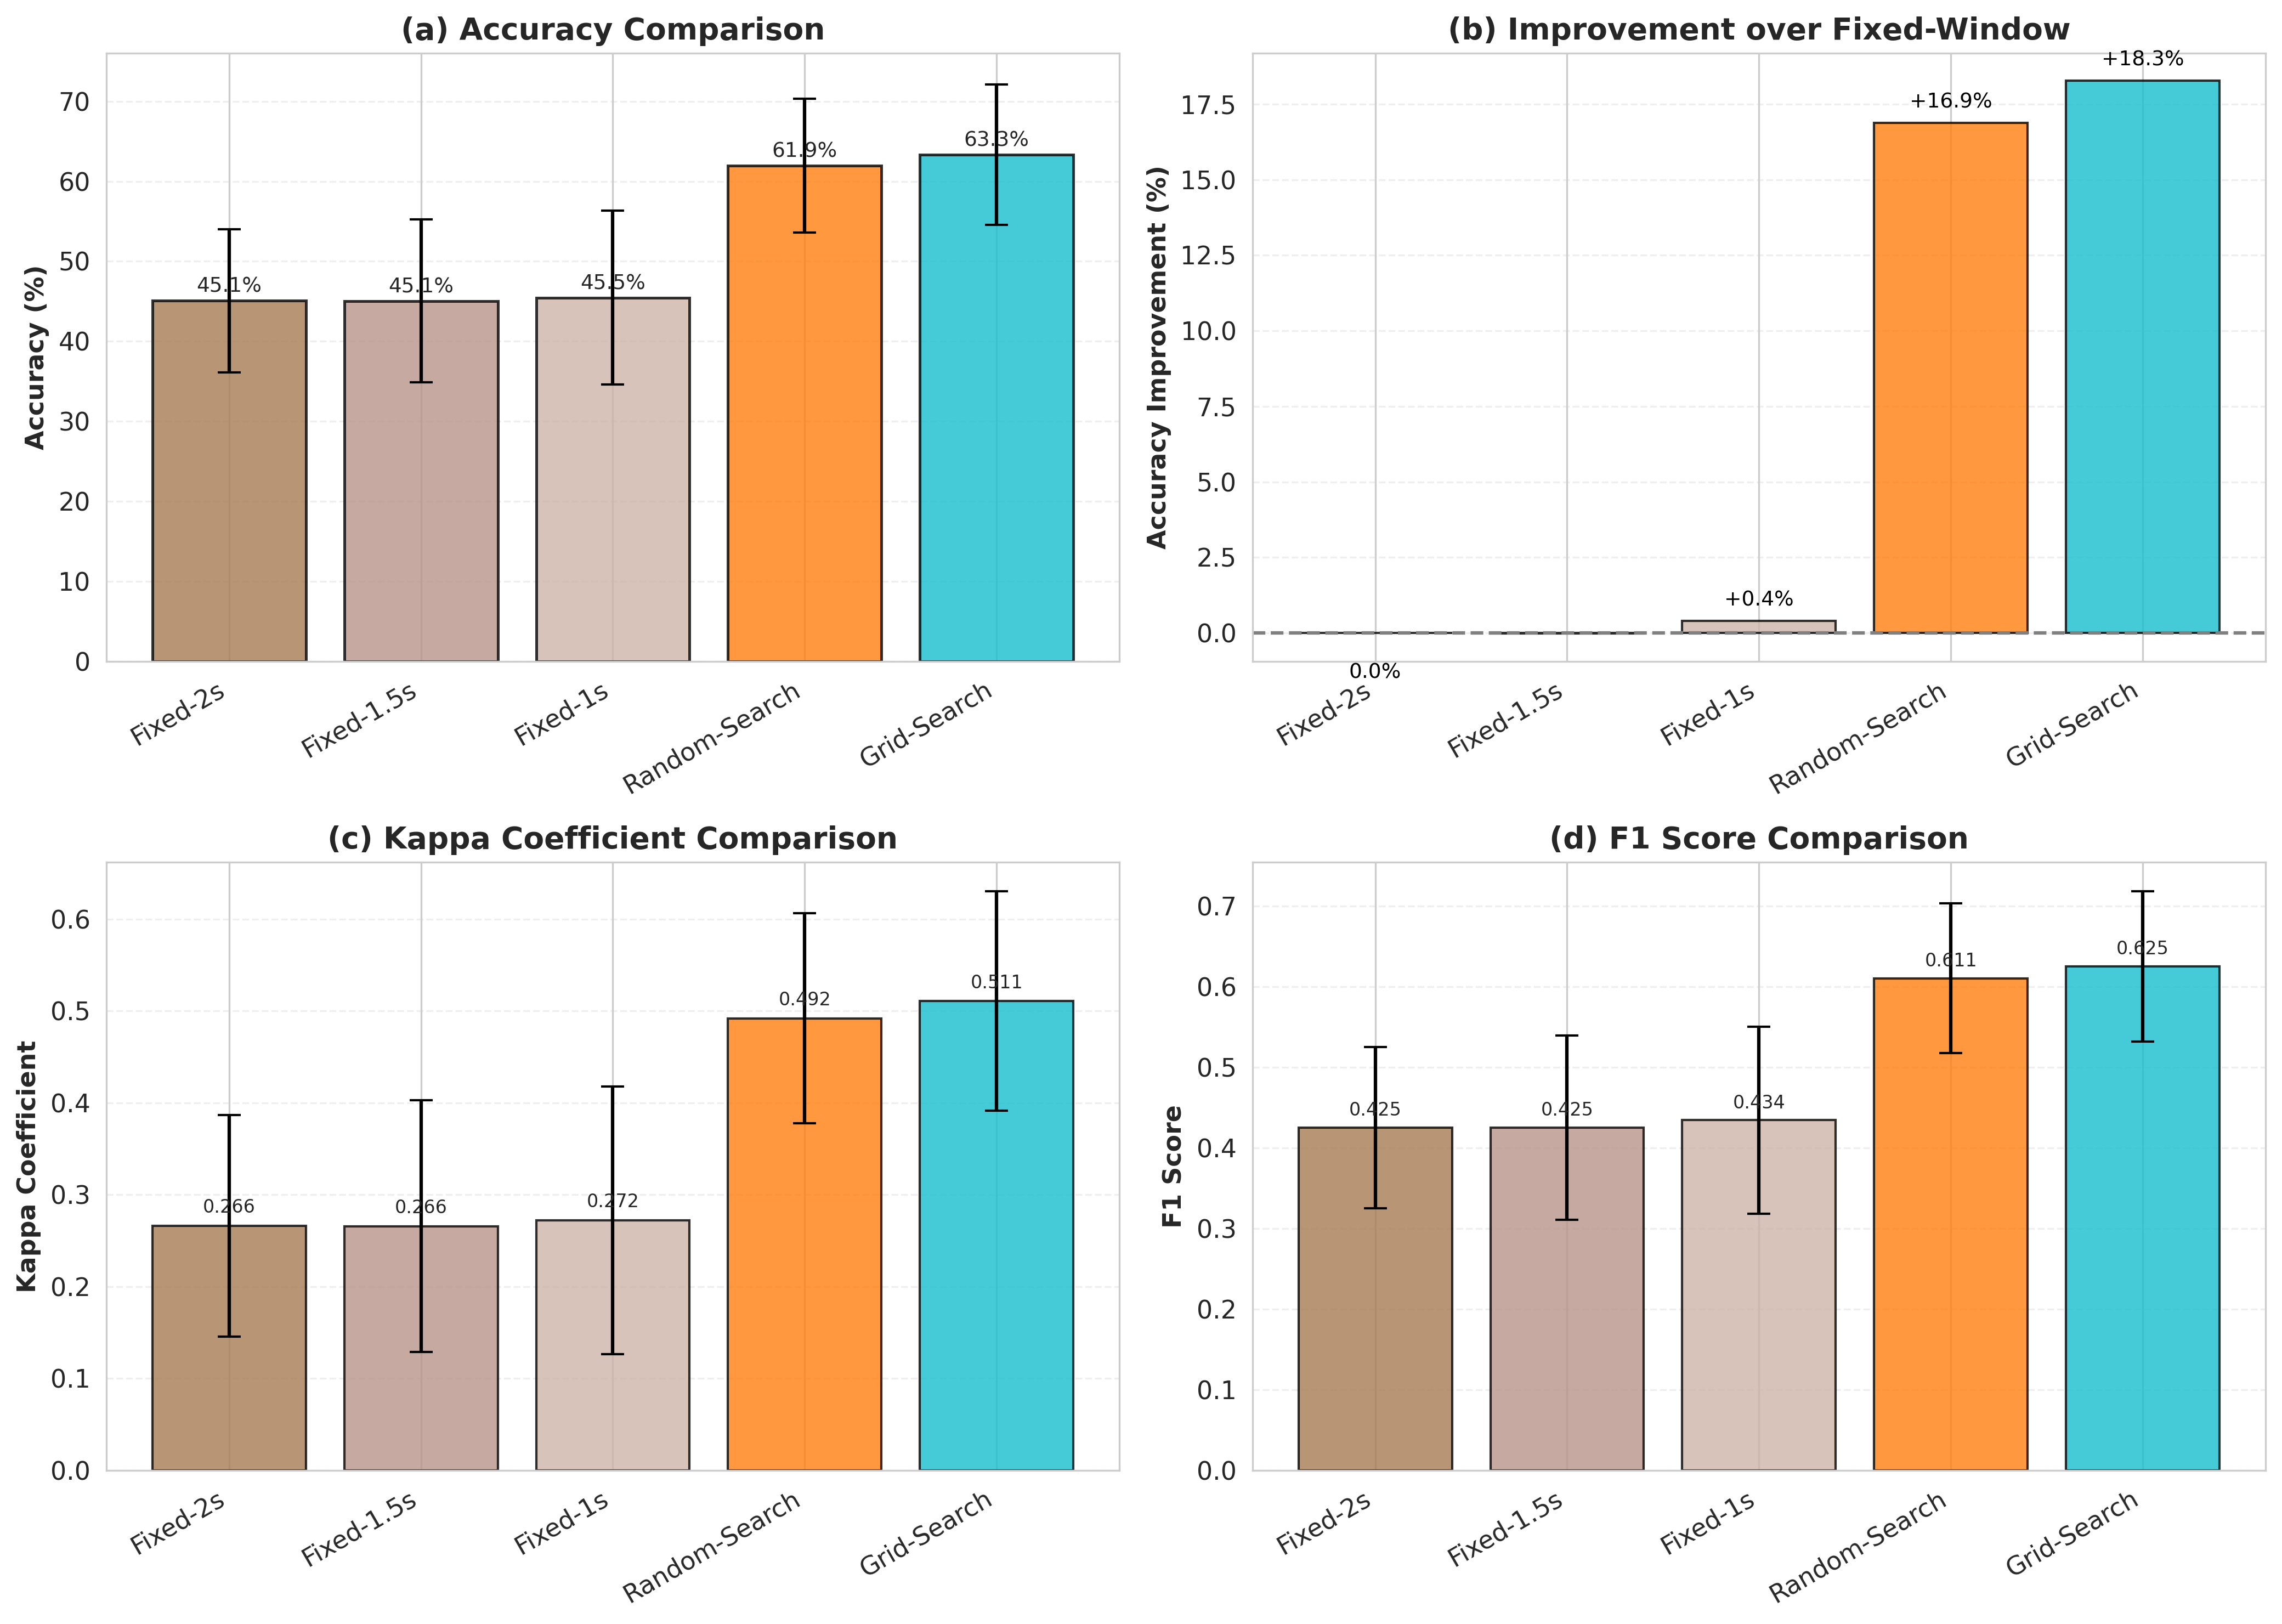
\includegraphics[width=1.0\textwidth]{figures/baseline/01_performance_comparison.png}
\caption{\textbf{基线方法的性能指标对比分析。}}
\label{fig:baseline_comparison}
\end{figure}

本图系统比较了固定窗口策略（Fixed-2s, Fixed-1.5s, Fixed-1s）与自适应搜索策略（Random-Search, Grid-Search）在多项分类性能指标上的表现。

\textbf{(a)} 分类准确率对比，误差线表示标准差。搜索策略（Random-Search: 61.9\%, Grid-Search: 63.3\%）显著优于固定窗口策略（约 45\%）。

\textbf{(b)} 相对于基准方法（Fixed-2s）的准确率提升百分比。Grid-Search 和 Random-Search 分别实现了 +18.3\% 和 +16.9\% 的显著提升，而 Fixed-1s 仅有 +0.4\% 的边际改善。

\textbf{(c)} Cohen's Kappa 系数对比，用于评估分类一致性。搜索策略（Random-Search: 0.492, Grid-Search: 0.511）表现出中等程度的一致性，明显优于固定窗口策略（约 0.27）。

\textbf{(d)} F1 分数对比，综合考量精确率与召回率。搜索策略（Random-Search: 0.611, Grid-Search: 0.625）较固定窗口策略（约 0.43）提升了约 44\%。

实验结果证实，自适应时间窗口搜索策略在各项评估指标上均显著优于固定窗口方法，其中 Grid-Search 表现最佳。

图~\ref{fig:baseline_stability}展示了五个基线方法在准确性方面的统计特性对比。

\begin{figure}[H]
\centering
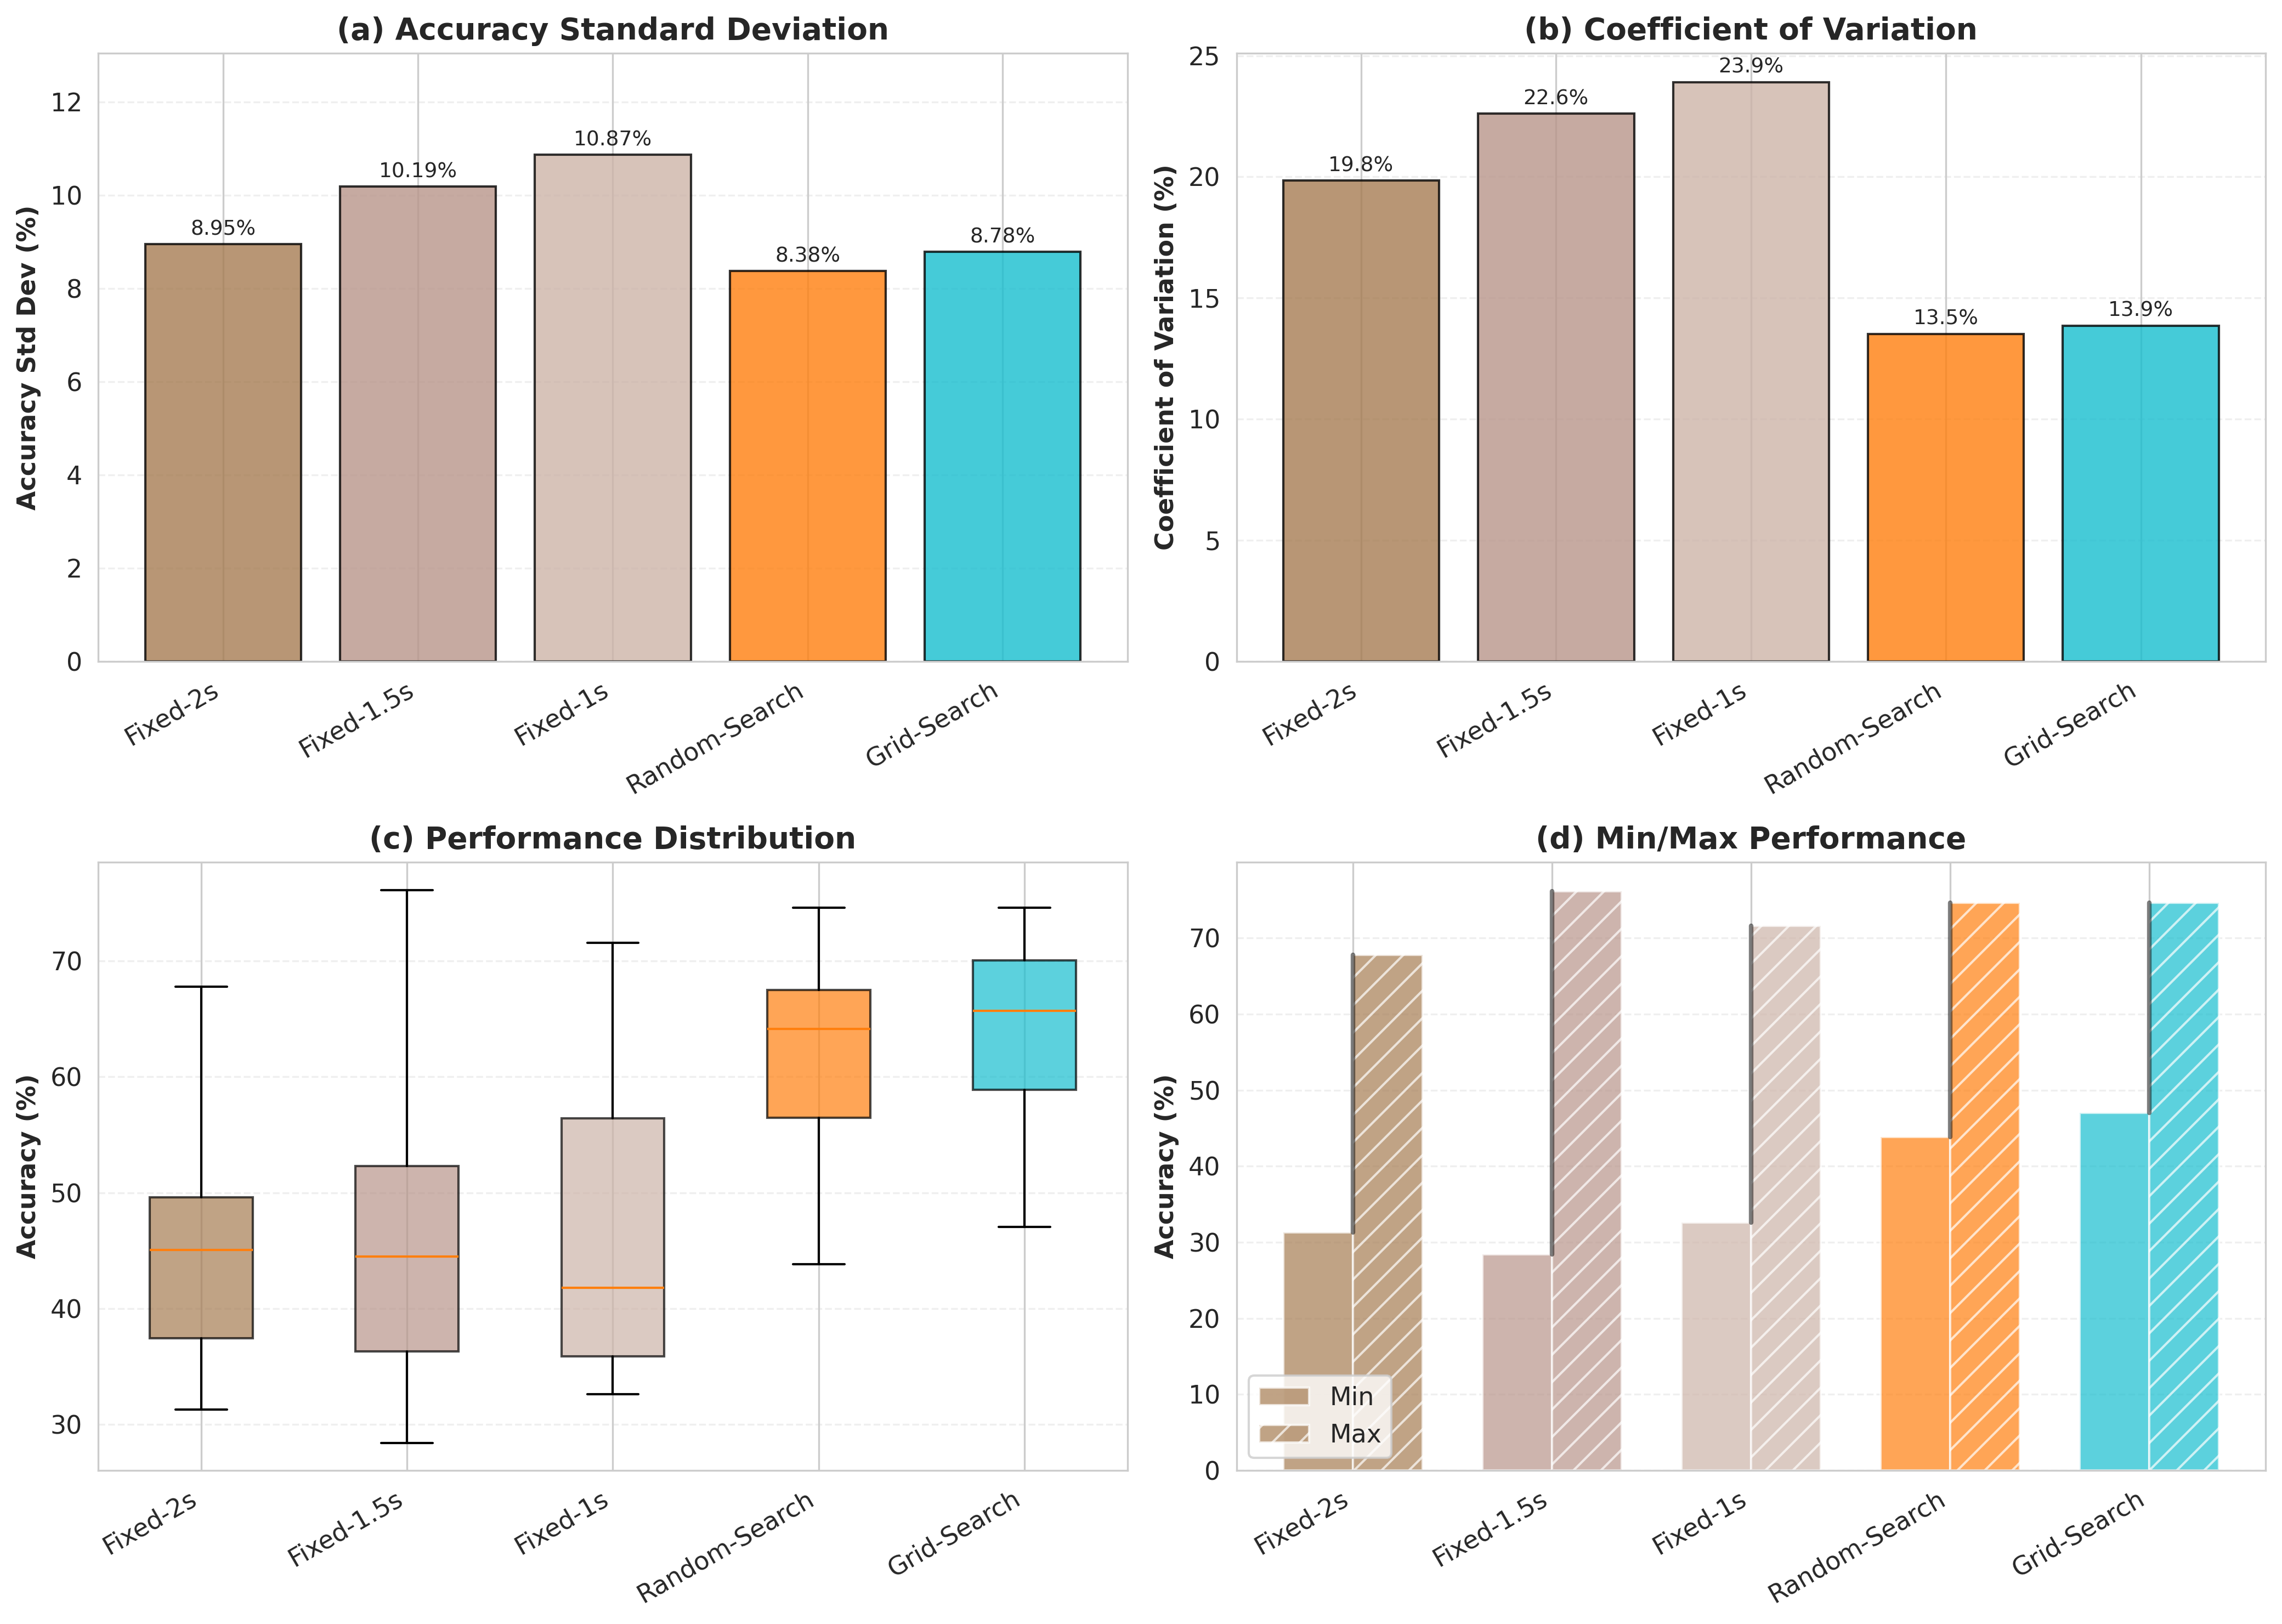
\includegraphics[width=1.0\textwidth]{figures/baseline/01_stability_analysis.png}
\caption{\textbf{基线方法的模型性能统计评估。} }
\label{fig:baseline_stability}
\end{figure}

本图综合评估了固定时长策略（Fixed-2s, Fixed-1.5s, Fixed-1s）与搜索优化策略（Random-Search, Grid-Search）在准确性指标上的表现。

\textbf{(a)} 准确性标准差，用于衡量预测结果的绝对波动性。如图所示，固定策略的标准差随时间窗口缩短呈递增趋势（从 8.95\% 升至 10.87\%）；而 Random-Search (8.38\%) 与 Grid-Search (8.78\%) 均低于所有固定配置，表明搜索机制有效平抑了单次运行中的随机震荡。

\textbf{(b)} 变异系数（CV），反映数据的相对离散程度。固定策略的 CV 普遍处于高位（19.8\%--23.9\%），尤其在 Fixed-1s 时相对离散风险最大；搜索策略则将该指标大幅压缩至 13.5\%--13.9\% 区间，证实了其跨实验批次具备更优的相对稳定性与可重复性。

\textbf{(c)} 准确性分布箱线图，展示中位数、四分位距及离群值分布。固定策略的箱体整体偏低且跨度较大（中位数集中于 42\%--45\%）；搜索策略不仅将分布中心显著上移（中位数跃升至 64\%--66\%），且箱体更为紧凑（尤以 Grid-Search 为甚），表明其高性能输出具有高度的一致性，有效压缩了低效区间的概率。

\textbf{(d)} 最小与最大准确性范围对比。固定策略的性能下限较低（Min 约 28\%--33\%），在实际部署中存在较大失效隐患；搜索策略通过参数寻优将下限显著抬升至 44\% 以上。同时，两者在峰值性能（Max）上表现相当（约 68\%--76\%），证明搜索策略在强化“保底能力”的同时，并未牺牲模型的性能上限。

实证结果表明，相较于固定时长策略，搜索策略在保持较高峰值性能的同时，显著降低了性能波动（较低的标准差和 CV），并提升了性能下限（较高的最小值和中位数），表现出更强的鲁棒性。

图~\ref{fig:subject_distribution}展示了五个基线方法在各被试实验的具体准确率表现。

\begin{figure}[H]
\centering
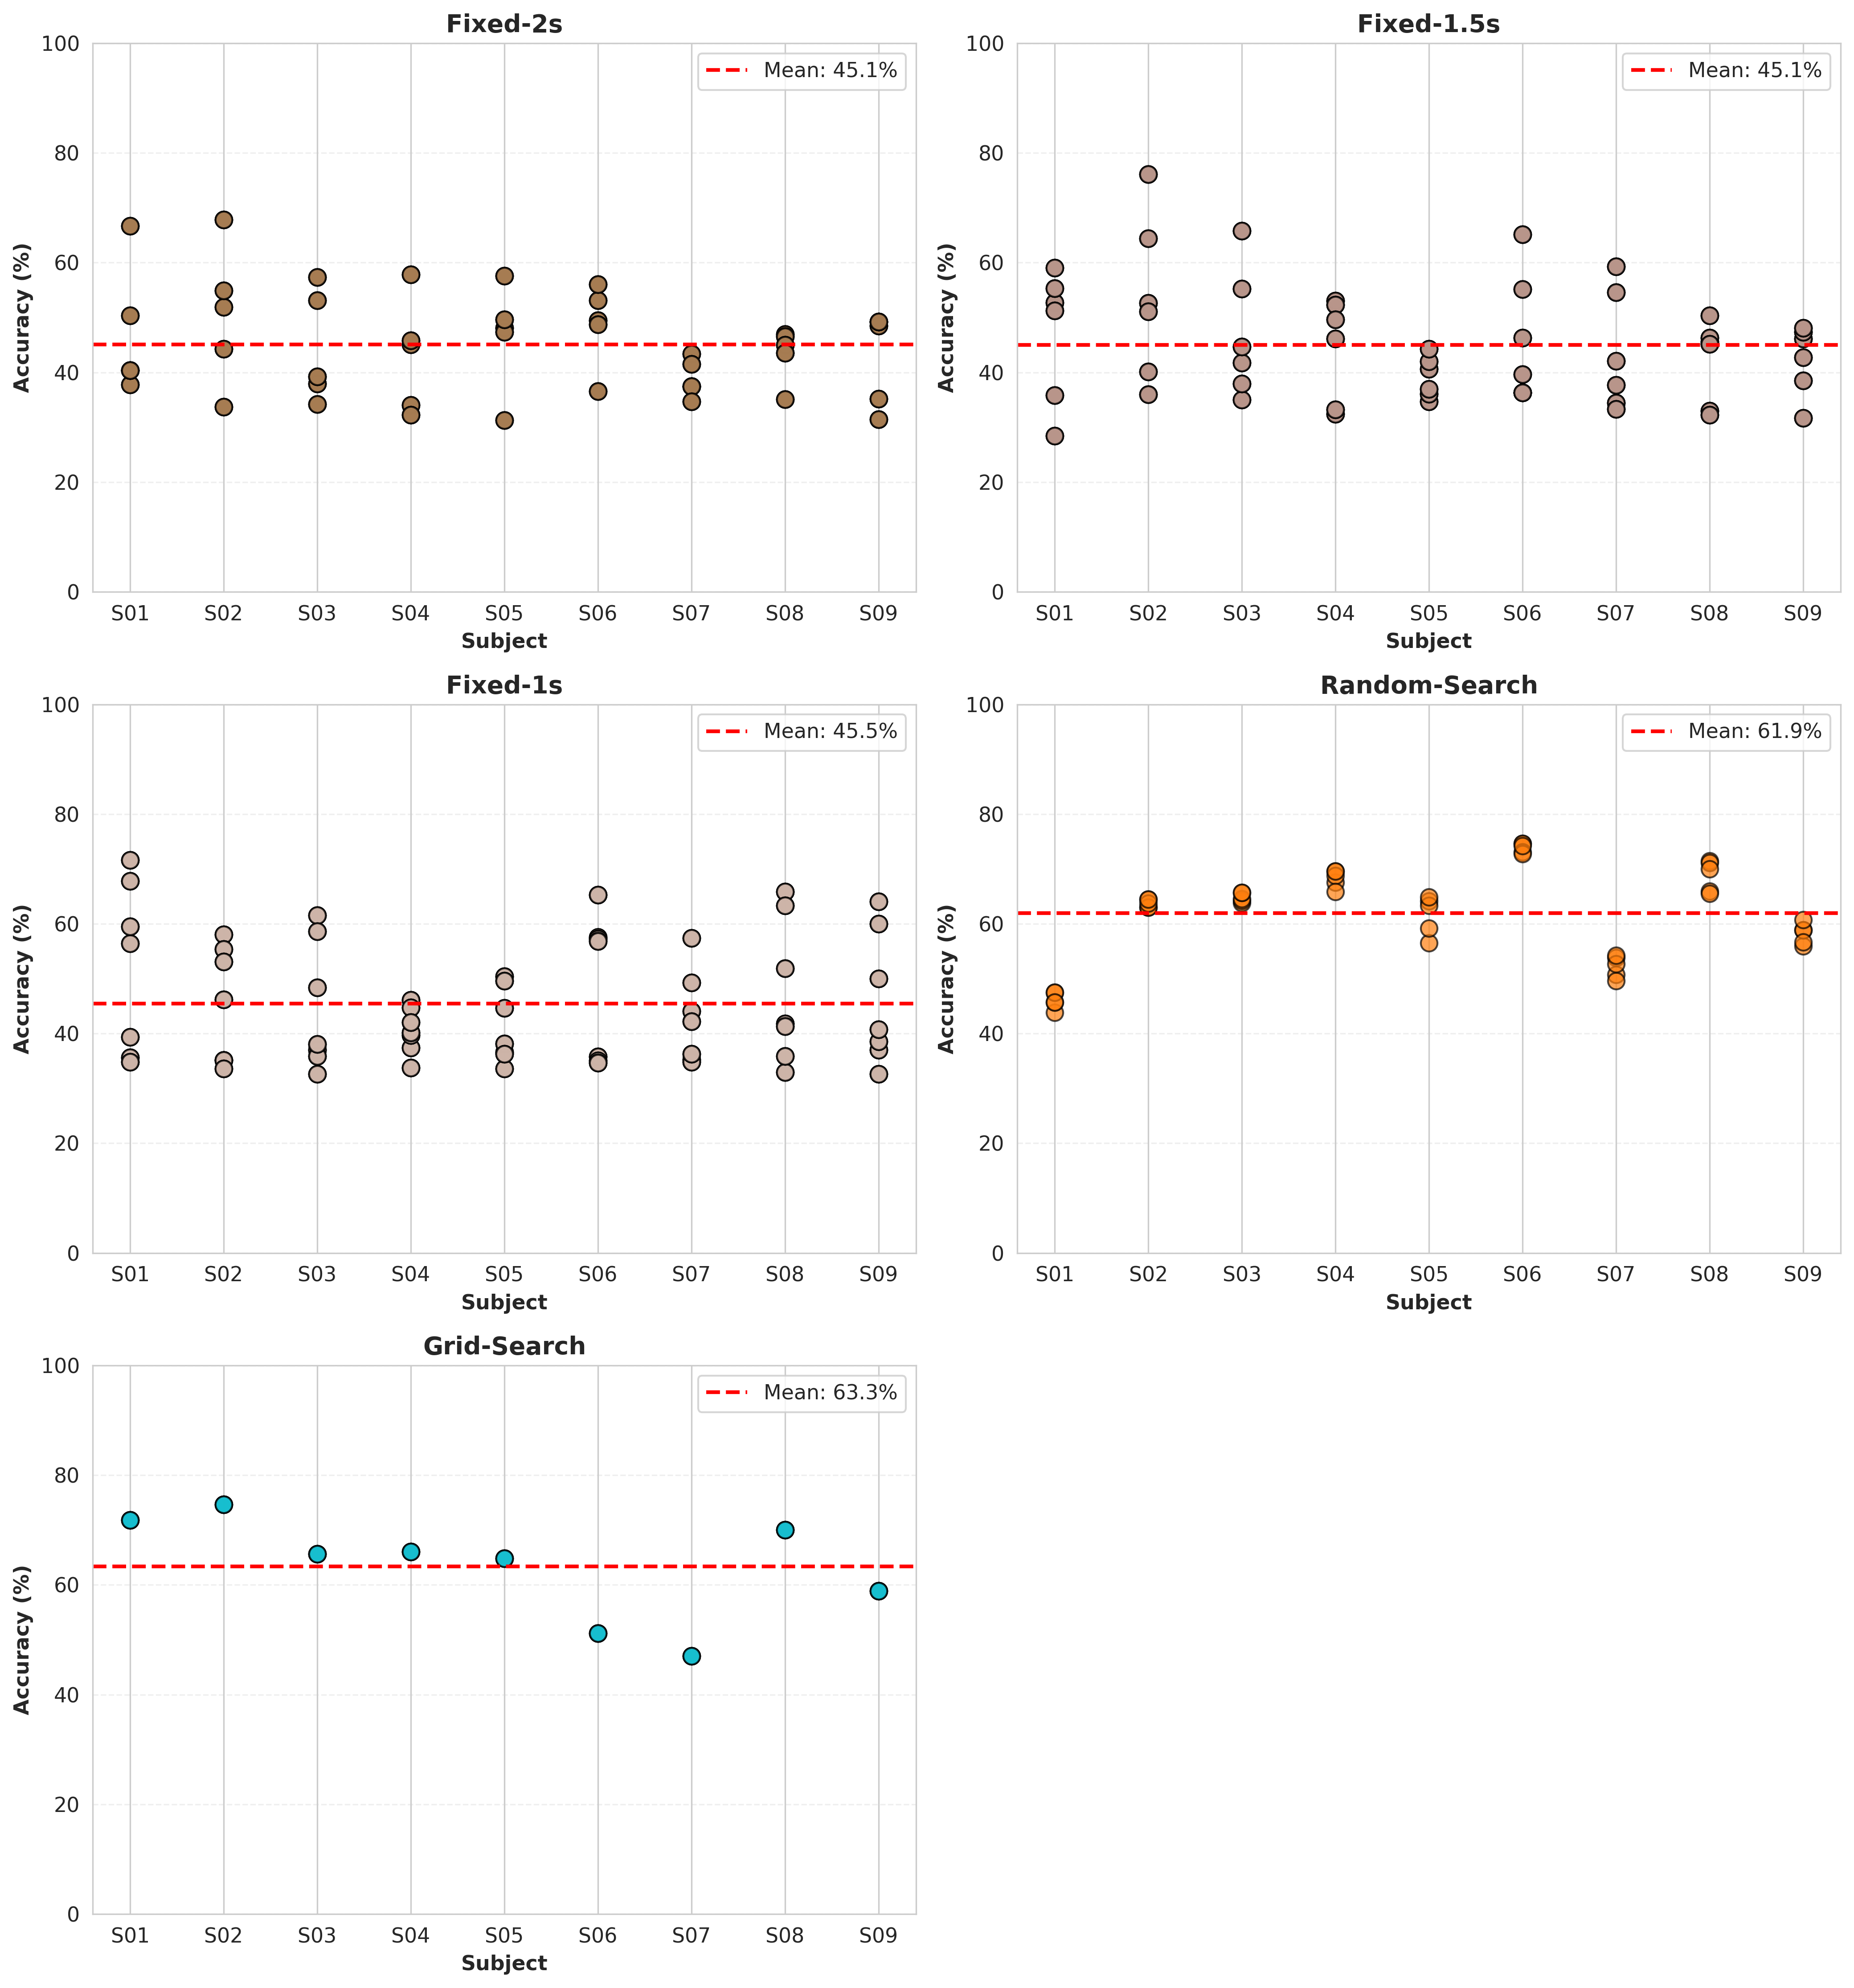
\includegraphics[width=1.0\textwidth]{figures/baseline/01_subject_distribution.png}
\caption{\textbf{不同时间窗口策略在各被试（Subjects S01--S09）上的准确率分布散点图。} }
\label{fig:subject_distribution}
\end{figure}

每个子图代表一种实验配置，散点表示单个被试的实验结果，红色虚线表示整体平均准确率。

\textbf{(a)--(c)} 固定窗口策略（Fixed-2s, Fixed-1.5s, Fixed-1s）表现出显著的被试间差异性（Inter-subject variability），数据点在纵轴方向分布广泛（范围约 30\%--70\%），且平均准确率停滞在 45\% 左右。

\textbf{(d)} Random-Search 策略显示出卓越的稳定性，同一被试的多次运行结果（每列多个点）高度聚集，且整体均值显著提升至 61.9\%。

\textbf{(e)} Grid-Search 策略取得了最高的平均准确率（63.3\%）。

结果表明，相较于固定窗口方法，基于搜索的优化策略不仅显著提升了分类性能，还有效缓解了个体差异带来的性能波动，展现了更强的鲁棒性。

表~\ref{tab:baseline_comparison} 展示了详细数值结果，包括准确率、Kappa 系数、F1 分数、标准差、变异系数。

\begin{table}[H]
\centering
\caption{基线方法性能比较}
\label{tab:baseline_comparison}
\small
\begin{tabular}{lccccc}
\hline
\textbf{Method} & \textbf{Accuracy (\%)} & \textbf{Kappa} & \textbf{F1} & \textbf{Std Dev (\%)} & \textbf{CV (\%)} \\
\hline
Fixed-2s & 45.08 $\pm$ 8.95 & 0.2662 $\pm$ 0.1204 & 0.4255 $\pm$ 0.1000 & 8.95 & 19.85  \\
Fixed-1.5s & 45.05 $\pm$ 10.19 & 0.2659 $\pm$ 0.1370 & 0.4253 $\pm$ 0.1142 & 10.19 & 22.61  \\
Fixed-1s & 45.47 $\pm$ 10.87 & 0.2721 $\pm$ 0.1456 & 0.4344 $\pm$ 0.1163 & 10.87 & 23.91  \\
Random-Search & 61.95 $\pm$ 8.38 & 0.4920 $\pm$ 0.1141 & 0.6106 $\pm$ 0.0930 & 8.38 & 13.52  \\
Grid-Search & \textbf{63.35 $\pm$ 8.78} & \textbf{0.5107 $\pm$ 0.1195} & \textbf{0.6252 $\pm$ 0.0932} & 8.78 & 13.86  \\
\hline
\end{tabular}
\end{table}

\xmusubsection{结果分析}{Result Analysis}
\label{subsec:results_analysis}

综合实验结果，主要发现如下：

\textbf{性能提升}： 搜索优化方法显著优于固定窗口策略。Grid-Search 准确率达 63.35\%，较 Fixed-2s 提升 18.3\%（相对提升 40.6\%）。Kappa 系数从 0.27 提升至 0.51，F1 分数从 0.43 提升至 0.63。这表明\textbf{自适应时间窗口能有效捕捉最优信号片段}，克服固定窗口无法适应 EEG 信号动态变化的局限。

\textbf{稳定性改善}： 尽管搜索方法的绝对标准差与 Fixed-2s 相近，但其变异系数显著降低（13.5\%--13.9\% vs 19.8\%--23.9\%）。更重要的是，搜索方法的最小准确率（约 47\%）远高于固定窗口（约 28\%--33\%），\textbf{有效避免了极端差性能的出现}，提高了方法的下限保障。

\textbf{个体差异适应}： 固定窗口方法在被试间表现出极大波动（30\%--70\%），而 Random-Search 在同一被试的多次运行中高度一致。这验证了\textbf{个体间神经响应模式的异质性}，搜索策略通过为每个样本独立优化窗口，有效适应了这种差异。

\textbf{搜索策略比较}： Grid-Search 略优于 Random-Search（+1.4\%），但差异微小（< 2.3\%）。考虑到 Random-Search 的计算效率优势，\textbf{在实时 BCI 系统中可能更具实用价值}。

\textbf{固定窗口局限}： 三种固定窗口长度性能几乎相同（45.05\%--45.47\%），表明\textbf{简单调整窗口长度无法解决固定窗口的固有局限}，自适应策略是必然选择。


\xmusection{Q-Learning 方法与基线方法对比分析}{Comparative Analysis of Q-Learning and Baselines}
\label{sec:ql_results}

\xmusubsection{整体性能对比}{Overall Performance Comparison}
\label{subsec:overall_comparison}

在验证自适应策略有效性的基础上，本节将 Q-Learning 方法族（Standard Q-Learning、Double Q-Learning、Dueling Q-Learning、Dueling Double Q-Learning、DQN）与基线方法（Grid-Search、Random-Search）进行系统对比。

图~\ref{fig:ql_baseline_comparison} 展示了所有方法的整体性能对比。

\begin{figure}[H]
\centering
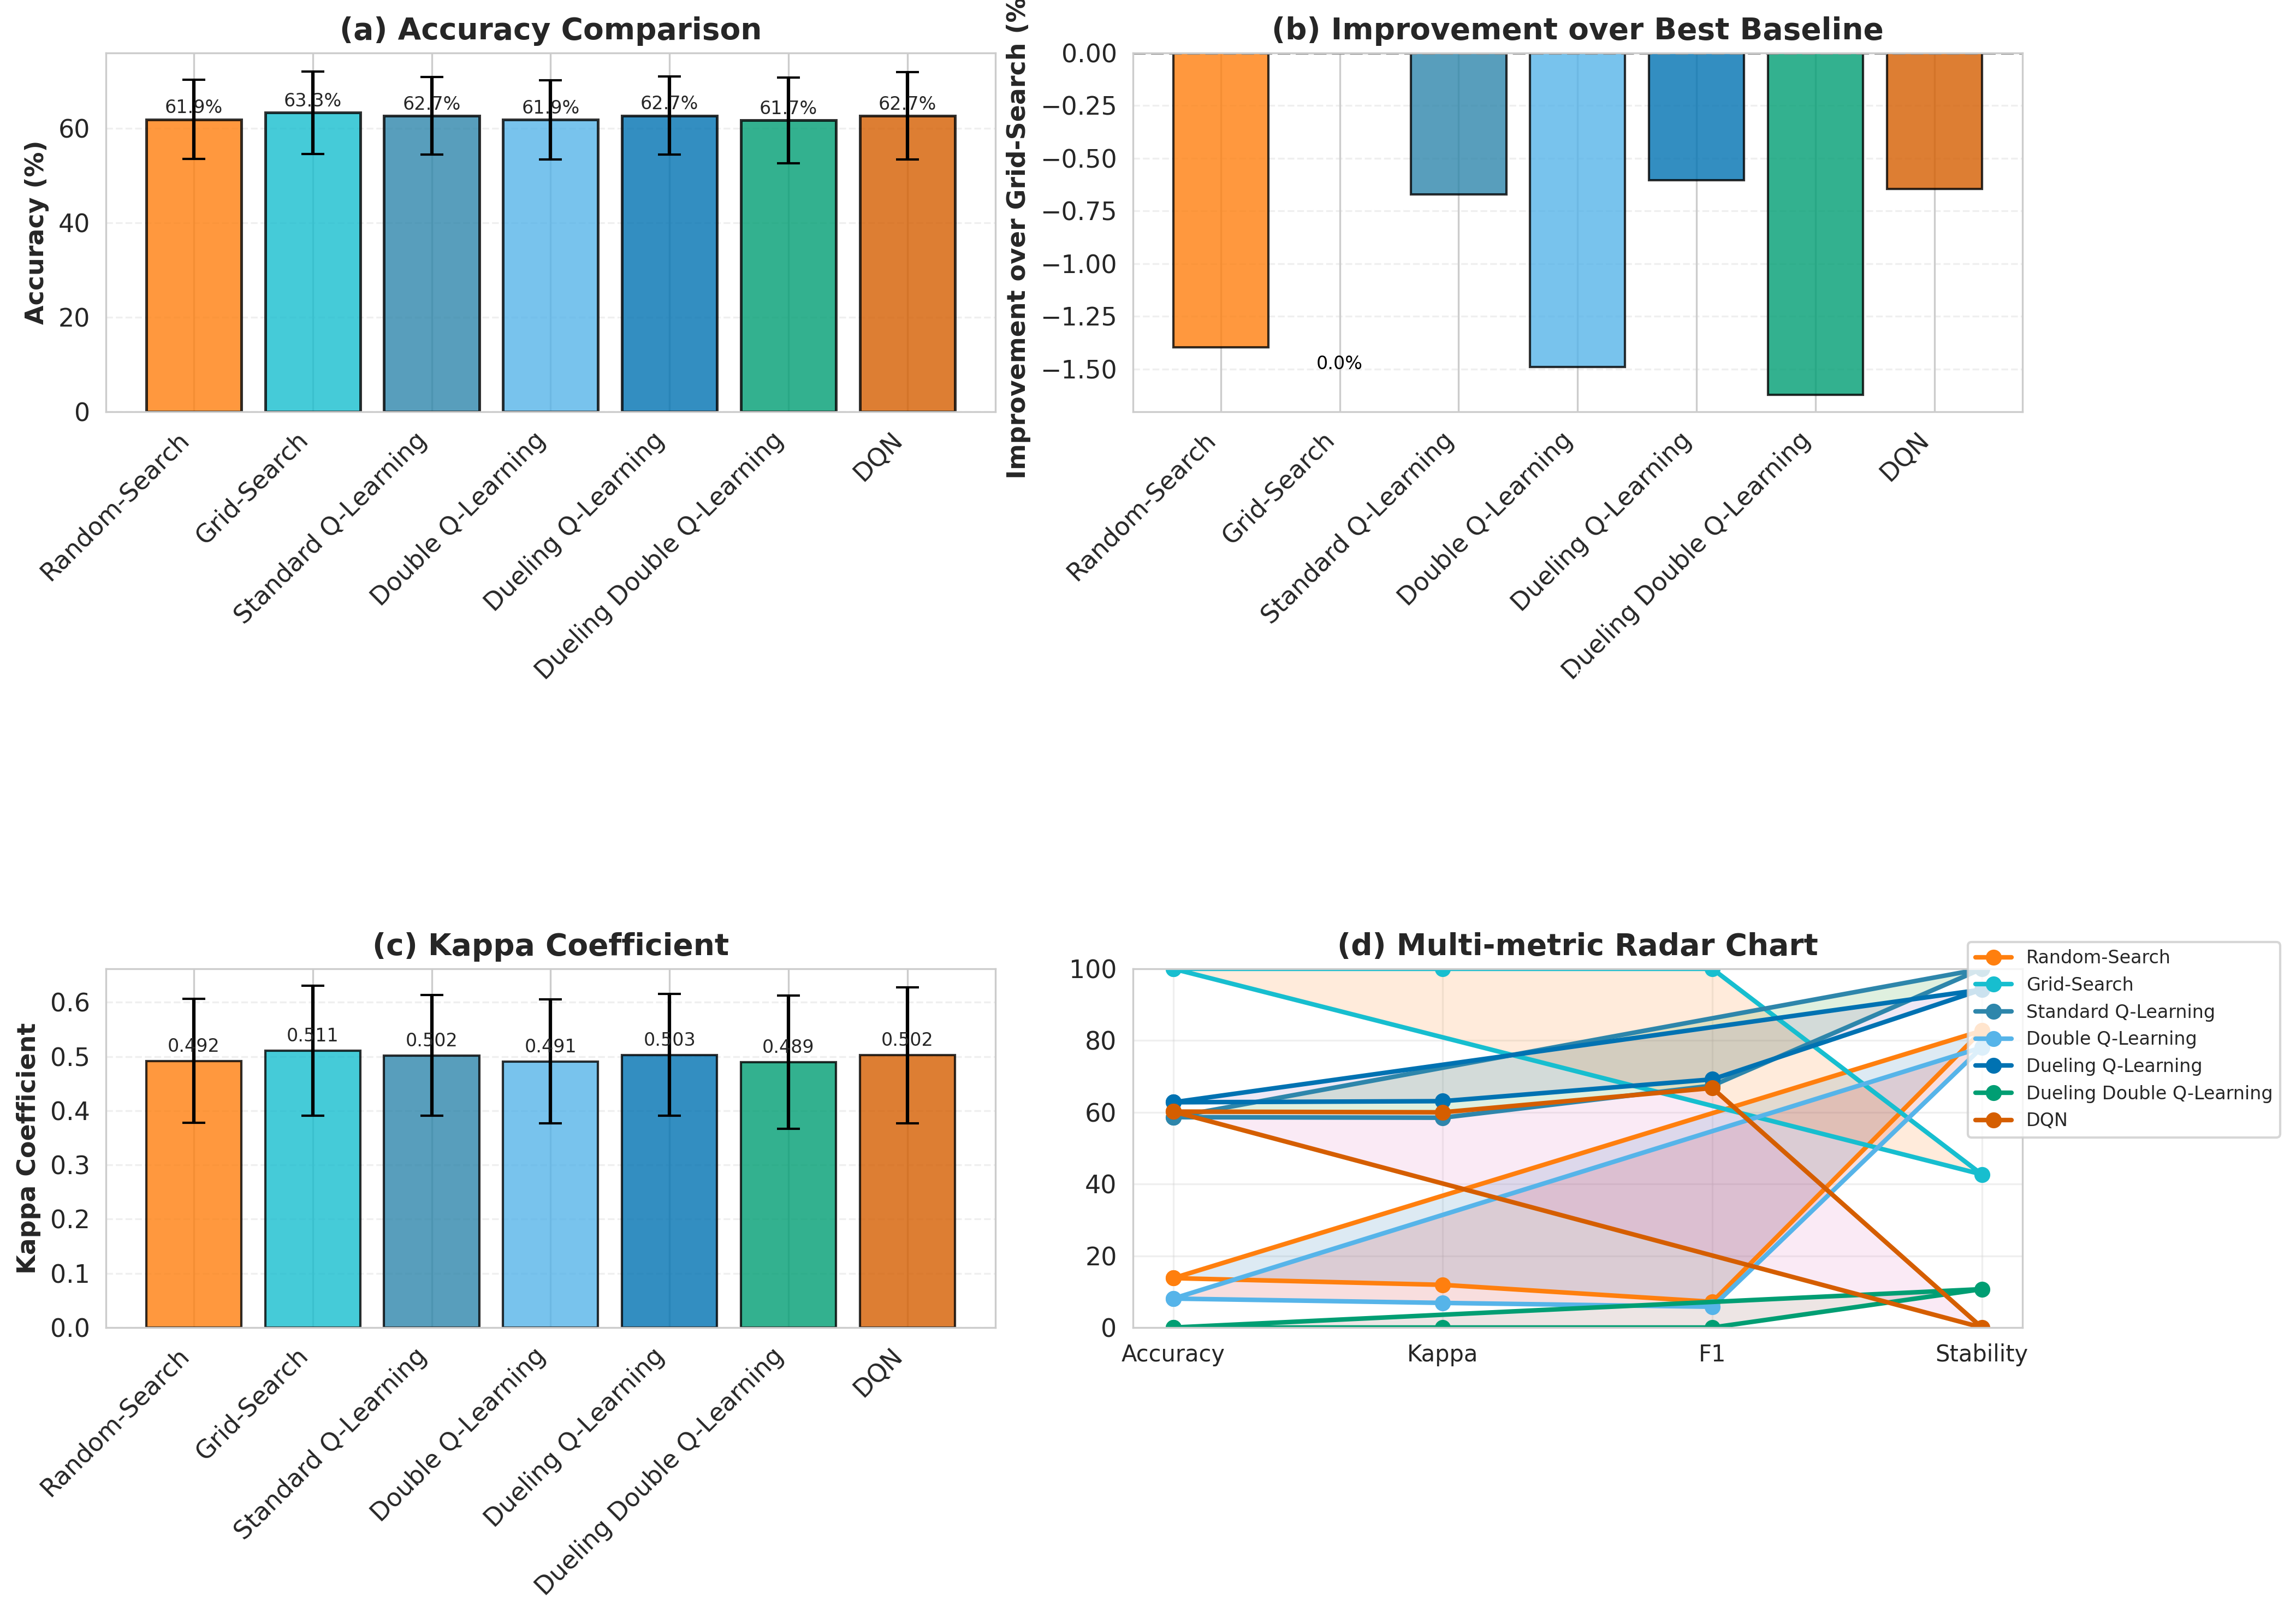
\includegraphics[width=1.0\textwidth]{figures/q_vs_baseline/02_performance_comparison.png}
\caption{\textbf{搜索优化方法与强化学习方法的性能对比分析。}}
\label{fig:ql_baseline_comparison}
\end{figure}

本图系统比较了搜索策略与多种强化学习策略在时间窗口选择任务上的表现。

\textbf{(a)} 分类准确率对比。所有方法性能相近（61.7\%--63.3\%），Grid-Search 以 63.3\% 略居首位。

\textbf{(b)} 相对于最佳基线（Grid-Search）的准确率改进。所有强化学习方法的性能均略低于 Grid-Search（-0.6\% 至 -1.6\%），Random-Search 差距为 -1.4\%。

\textbf{(c)} Cohen's Kappa 系数对比。各方法 Kappa 系数集中在 0.49--0.51 之间，分类一致性水平相当。

\textbf{(d)} 多指标雷达图，综合展示准确率、Kappa 系数、F1 分数和稳定性（变异系数倒数归一化）。Grid-Search 在准确率和 F1 分数上表现最优，而部分强化学习方法在稳定性指标上略有优势。

实验结果表明，强化学习方法能够以较低的计算成本达到与网格搜索相近的性能水平，为实时自适应时间窗口选择提供了可行方案。

图~\ref{fig:ql_statistical} 展示了Q-Learning方法与基线方法的统计分析。

\begin{figure}[H]
\centering
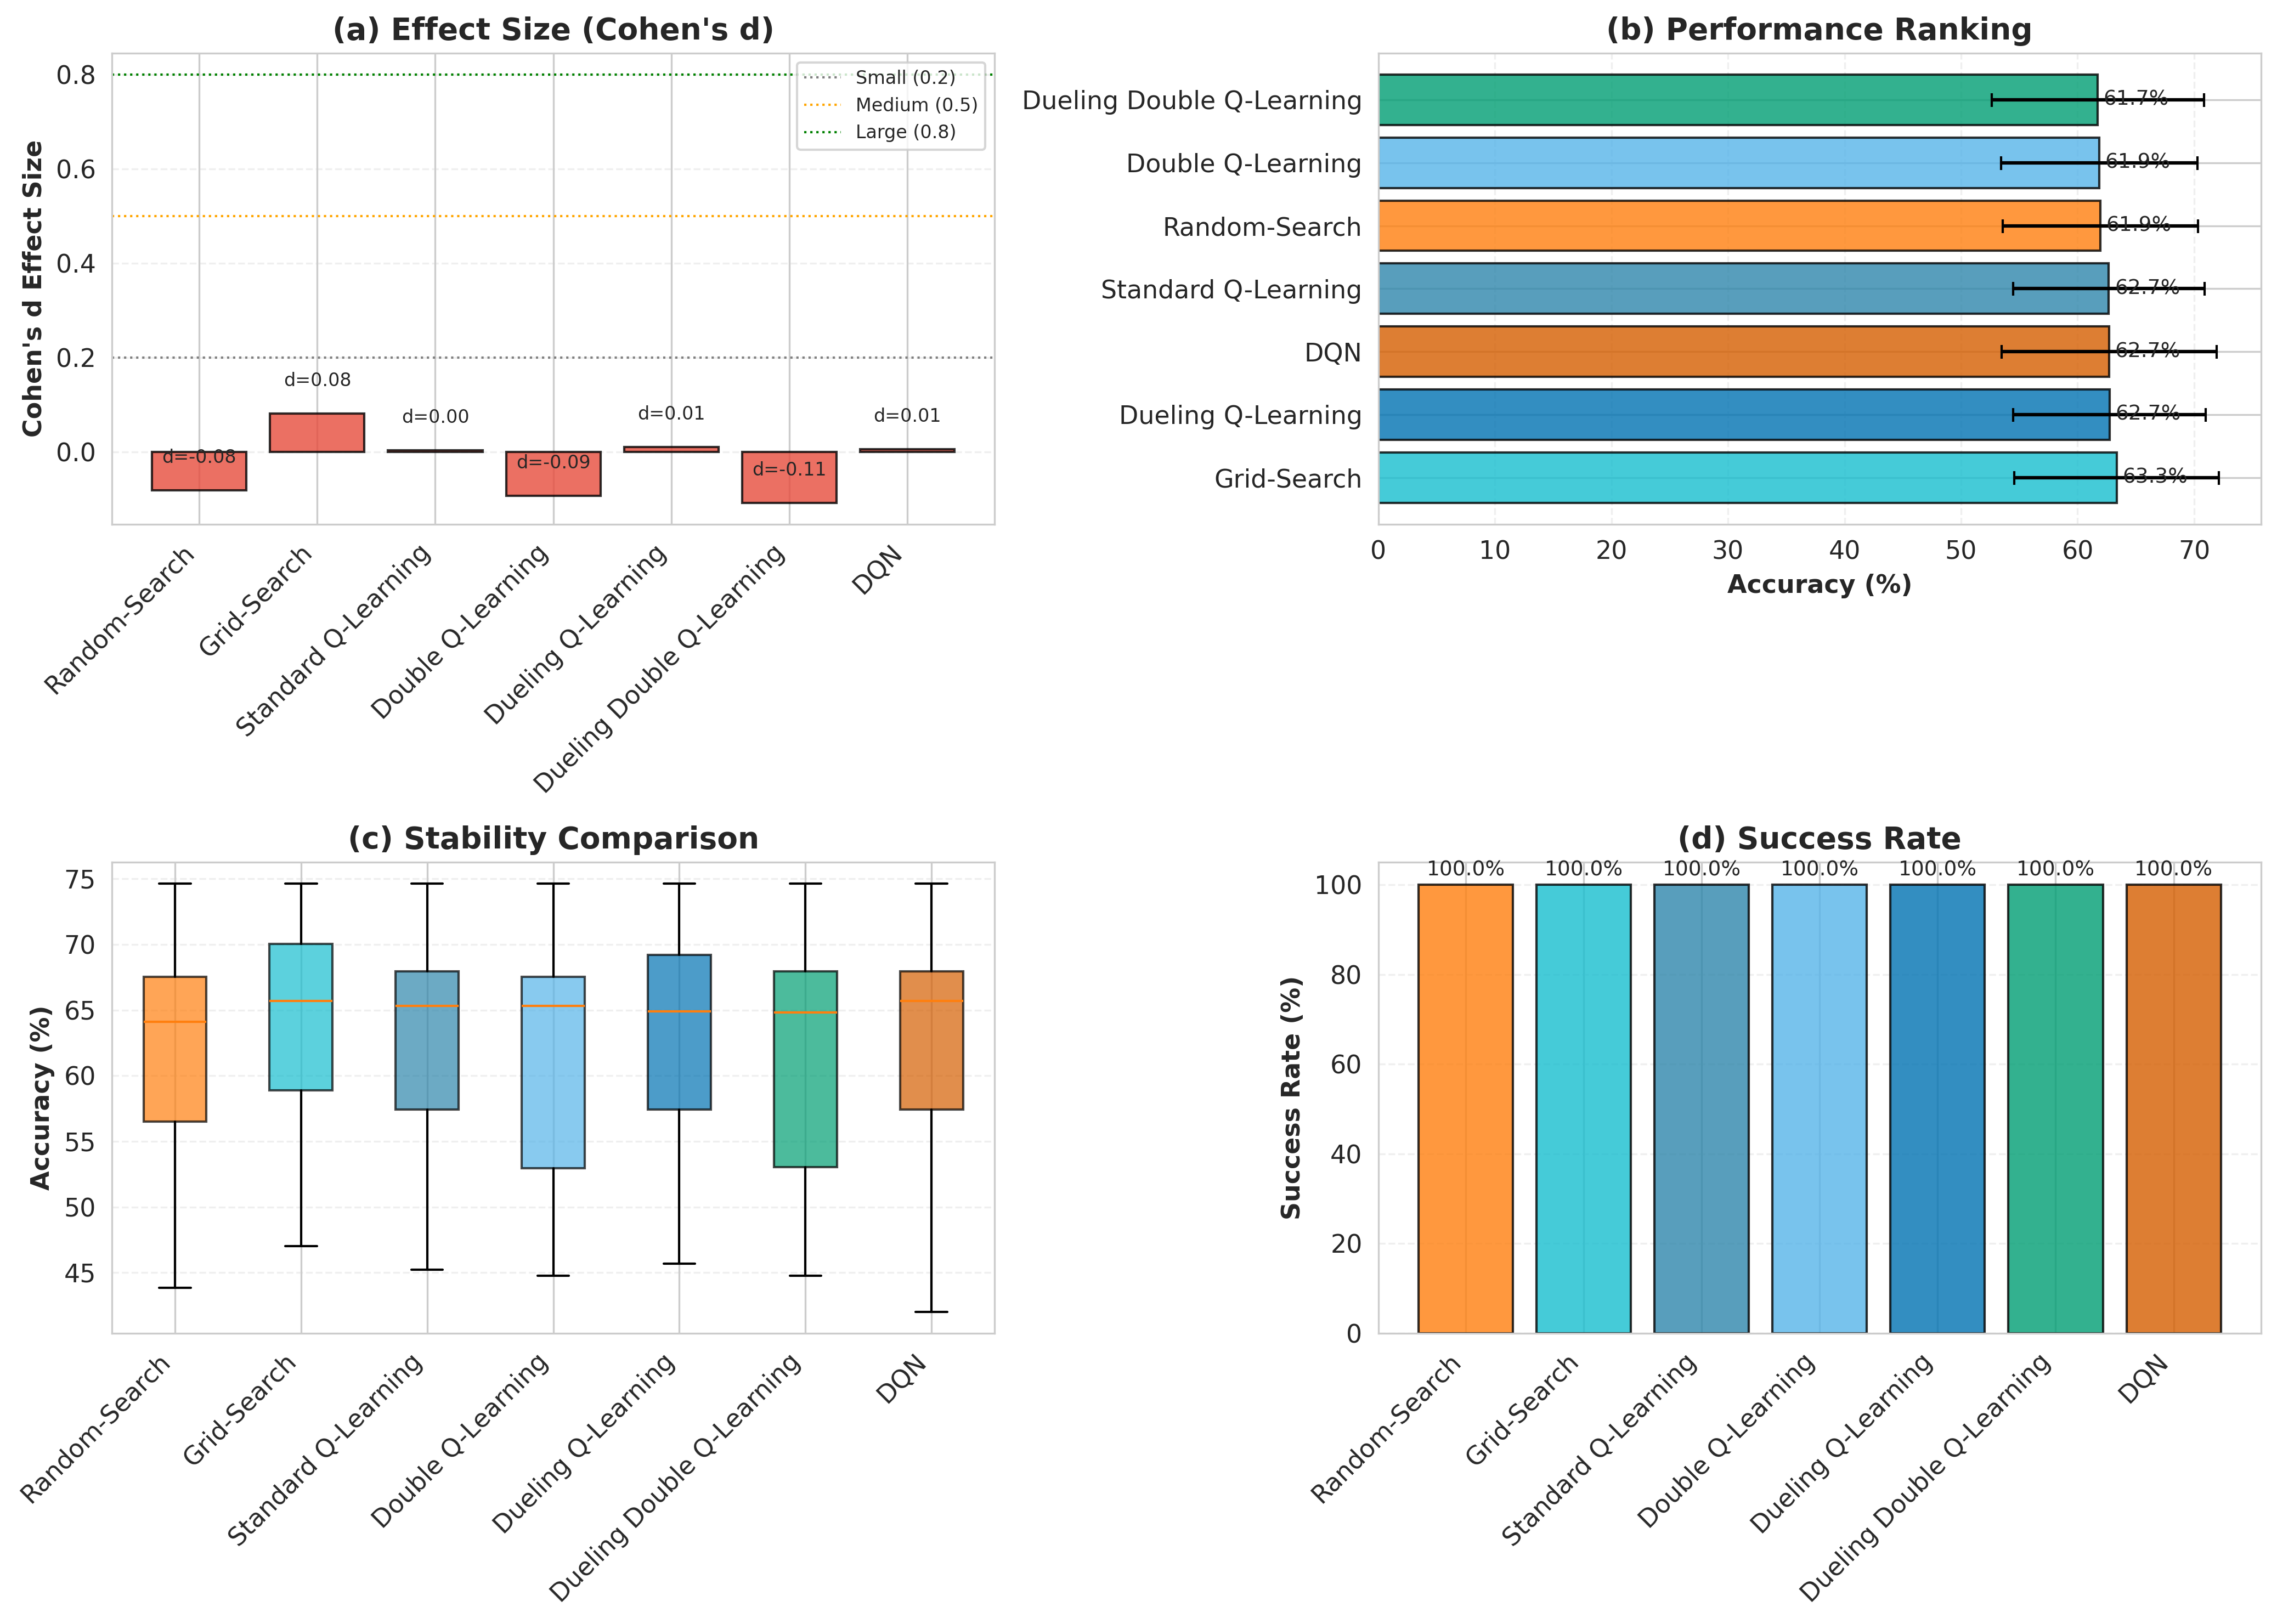
\includegraphics[width=1.0\textwidth]{figures/q_vs_baseline/02_statistical_analysis.png}
\caption{\textbf{搜索优化与强化学习方法的统计显著性分析。}}
\label{fig:ql_statistical}
\end{figure}

本图从效应量、性能排名、稳定性和成功率四个维度对七种时间窗口选择方法进行了全面的统计评估。

\textbf{(a)} Cohen's d 效应量分析，以 Grid-Search 为基准。所有方法的效应量均远小于小效应阈值（$|d| < 0.2$），其中 Random-Search ($d=-0.08$)、Dueling Double Q-Learning ($d=-0.11$) 和 Double Q-Learning ($d=-0.09$) 显示出微小的负效应，表明这些方法性能略低于 Grid-Search，但差异不显著。

\textbf{(b)} 性能排名对比。Grid-Search 以 63.3\% 的准确率位居首位，Dueling Q-Learning、DQN 和 Standard Q-Learning 并列第二（62.7\%），Random-Search 和 Double Q-Learning 紧随其后（61.9\%），Dueling Double Q-Learning 略低（61.7\%）。

\textbf{(c)} 稳定性对比箱线图。各方法的准确率分布范围相近（约 45\%--75\%），中位数集中在 65\% 左右，Grid-Search 和 Dueling Q-Learning 表现出略高的下四分位数。

\textbf{(d)} 成功率对比。所有方法均达到 100\% 的成功率，表明各方法在不同实验条件下均能稳定收敛。

综合分析表明，尽管 Grid-Search 在准确率上略有优势，但所有强化学习变体与其性能差异均不显著（Cohen's d $< 0.2$），验证了强化学习方法在保持性能的同时大幅降低计算成本的有效性。

\xmusubsection{时间窗选择分析}{Time Window Selection Analysis}
\label{subsec:window_analysis}

图~\ref{fig:window_analysis} 展示了各方法选择的时间窗位置及窗口长度与性能的关系。

\begin{figure}[H]
\centering
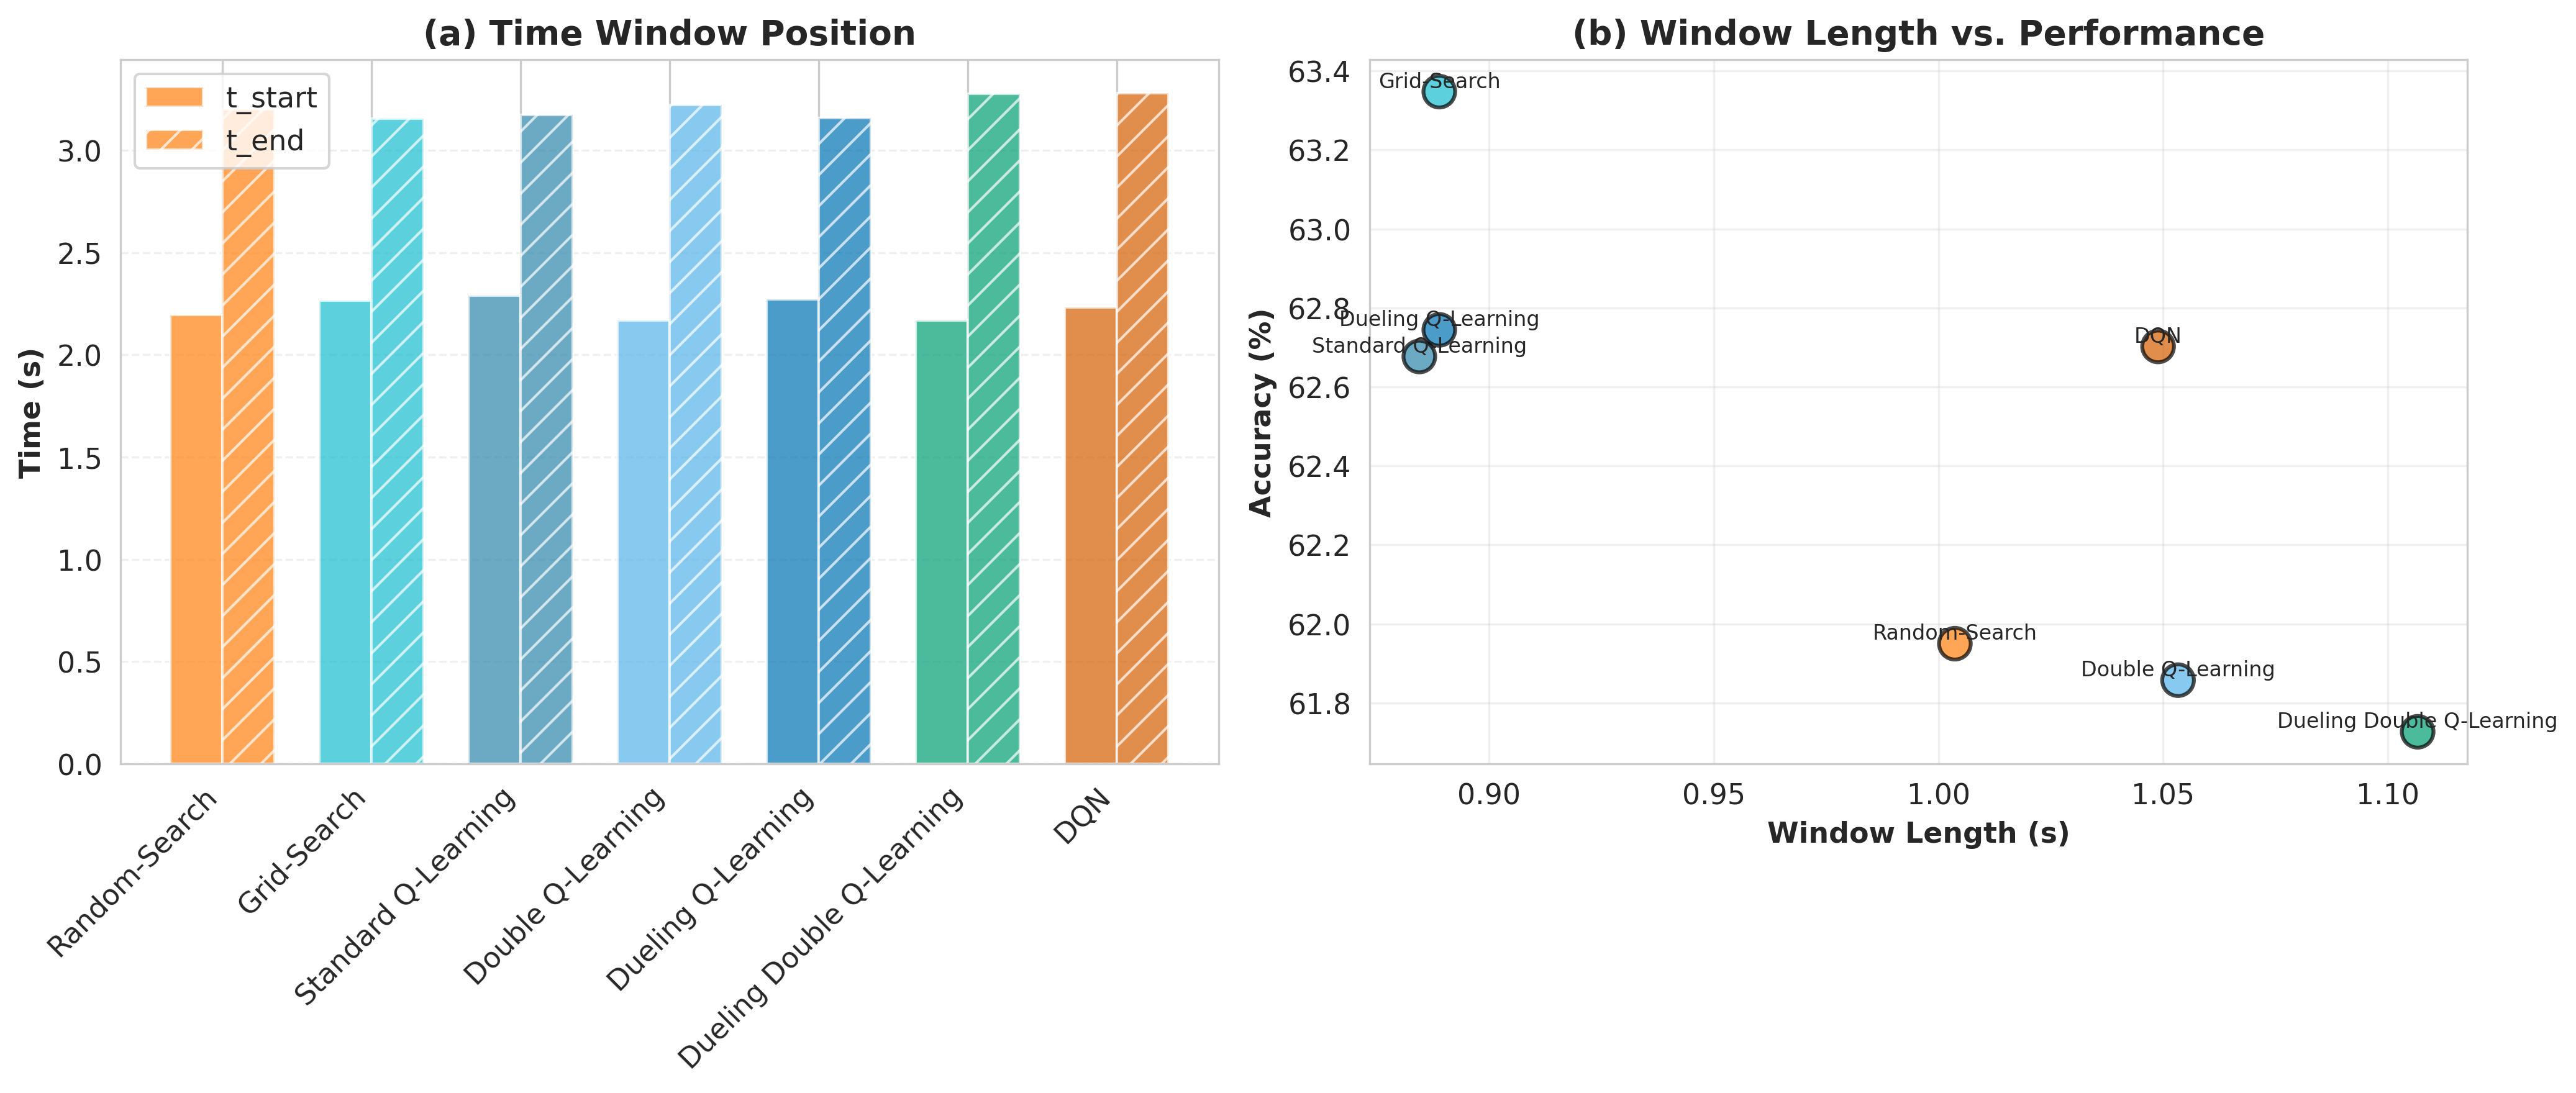
\includegraphics[width=1.0\textwidth]{figures/q_vs_baseline/02_window_performance.png}
\caption{\textbf{时间窗口选择模式与性能关系分析。}}
\label{fig:window_analysis}
\end{figure}

\textbf{(a)} 时间窗口位置分布，展示了各方法选择的起始时间 ($t_{start}$) 和结束时间 ($t_{end}$)。观察发现，所有方法均倾向于选择试验后期的时间片段，起始时间集中在 2.2s--2.3s，结束时间在 3.2s--3.3s 之间。这一致性表明\textbf{运动想象任务相关的关键神经特征主要分布在 trials 的后半段}。

\textbf{(b)} 窗口长度与分类准确率的关系散点图。结果显示窗口长度与性能存在潜在的负相关趋势：较短的窗口（约 0.9s，如 Grid-Search 和部分 Q-Learning 变体）取得了更高的准确率（62.7\%--63.3\%），而较长窗口（>1.0s，如 Dueling Double Q-Learning）准确率略低（61.7\%）。Grid-Search 以 0.89s 的最短窗口实现了 63.3\% 的最高准确率，进一步证实了\textbf{精简时间窗口有助于减少无关噪声干扰并提升分类性能}，而强化学习代理在探索过程中也逐渐收敛至这一最优窗口长度附近。

表~\ref{tab:ql_comparison} 展示了各方法的详细性能数据。

\begin{table}[H]
\centering
\caption{Q-Learning 方法与基线方法详细对比}
\label{tab:ql_comparison}
\small
\begin{tabular}{lcccc}
\hline
\textbf{Method}  & \textbf{Accuracy (\%)} & \textbf{Kappa} & \textbf{F1} & \textbf{Std Dev (\%)}  \\
\hline
Random-Search  & 61.95 $\pm$ 8.38 & 0.4920 $\pm$ 0.1141 & 0.6106 $\pm$ 0.0930 & 8.38  \\
Grid-Search  & \textbf{63.35 $\pm$ 8.78} & \textbf{0.5107 $\pm$ 0.1195} & \textbf{0.6252 $\pm$ 0.0932} & 8.78  \\
Standard Q-Learning  & 62.68 $\pm$ 8.20 & 0.5019 $\pm$ 0.1114 & 0.6201 $\pm$ 0.0869 & \textbf{8.20}  \\
Double Q-Learning  & 61.86 $\pm$ 8.42 & 0.4909 $\pm$ 0.1143 & 0.6103 $\pm$ 0.0901 & 8.42  \\
Dueling Q-Learning  & 62.74 $\pm$ 8.26 & 0.5029 $\pm$ 0.1122 & 0.6204 $\pm$ 0.0873 & 8.26  \\
Dueling Double Q-Learning  & 61.73 $\pm$ 9.11 & 0.4894 $\pm$ 0.1231 & 0.6094 $\pm$ 0.0952 & 9.11  \\
DQN  & 62.70 $\pm$ 9.21 & 0.5022 $\pm$ 0.1251 & 0.6200 $\pm$ 0.0970 & 9.21  \\
\hline
\end{tabular}
\end{table}

\xmusubsection{结果分析}{Result Analysis}
\label{subsec:ql_analysis}

综合上述实验结果，对Q-Learning方法与基线方法的对比分析如下：

\textbf{性能对比}: Grid-Search以63.35\%的准确率位居首位，Q-Learning变体的准确率分布在61.73\%--62.74\%之间，与Grid-Search的差距仅为0.6\%--1.6\%。Standard Q-Learning和Dueling Q-Learning表现最佳（62.7\%），显著优于Random-Search（61.9\%）。Kappa系数和F1分数的趋势与准确率一致，所有方法的Kappa系数均处于0.49--0.51的中等一致性水平。

\textbf{统计显著性}: 所有Q-Learning方法与Grid-Search的Cohen's d值均远小于小效应阈值（$|d| < 0.2$），其中Dueling Double Q-Learning的效应量最大（$d=-0.11$）。这表明\textbf{尽管Grid-Search在数值上略优，但差异在统计学上不显著}，Q-Learning方法可视为与Grid-Search性能等效。

\textbf{时间窗口选择模式}: 所有方法均倾向于选择试验后期的时间片段（$t_{start} \approx 2.2$s，$t_{end} \approx 3.3$s），验证了运动想象关键特征分布在trials后半段的假设。此外，窗口长度与性能呈负相关趋势，较短窗口（约0.9s）比较长窗口（>1.0s）准确率更高，表明\textbf{精简窗口有助于减少噪声干扰}。Q-Learning代理在训练过程中逐渐收敛至这一最优窗口范围，体现了其学习能力。

\textbf{稳定性与计算效率}: 从标准差来看，Standard Q-Learning（8.20\%）和Dueling Q-Learning（8.26\%）的稳定性略优于Grid-Search（8.78\%）和Random-Search（8.38\%）。更重要的是，Q-Learning方法在推理阶段仅需单次前向传播即可确定时间窗口，而Grid-Search需要遍历所有候选窗口组合。考虑到两者性能差异不显著（$< 1.6\%$），\textbf{Q-Learning方法在实时BCI系统中具有明显的计算效率优势}。

\textbf{Q-Learning变体比较}: 在五种Q-Learning变体中，Standard Q-Learning和Dueling Q-Learning表现最佳，而Dueling Double Q-Learning略低（61.73\%）。这一结果与理论预期部分吻合：Dueling架构通过分离状态价值和优势函数提升了性能，但Double Q-Learning的过估计修正在本任务中收益有限，甚至可能因过度保守而略微降低性能。

\xmusection{表格型 Q-Learning 与 DQN 对比分析}{Comparative Analysis of Q-Learning and DQN}
\label{sec:tableq_vs_dqn}

\xmusubsection{整体性能对比}{Overall Performance Comparison}
\label{subsec:overall_tableq_dqn}

本节聚焦于表格型 Q-Learning 与 DQN 的详细对比，验证本研究的核心主张：\textbf{表格型 Q-Learning 可以在不显著牺牲性能的前提下替代 DQN}。

图~\ref{fig:tableq_dqn_comparison} 深入评估了五种 Q-Learning 变体（Standard, Double, Dueling, Dueling Double, DQN）在时间窗口选择任务上的表现差异。

\begin{figure}[H]
\centering
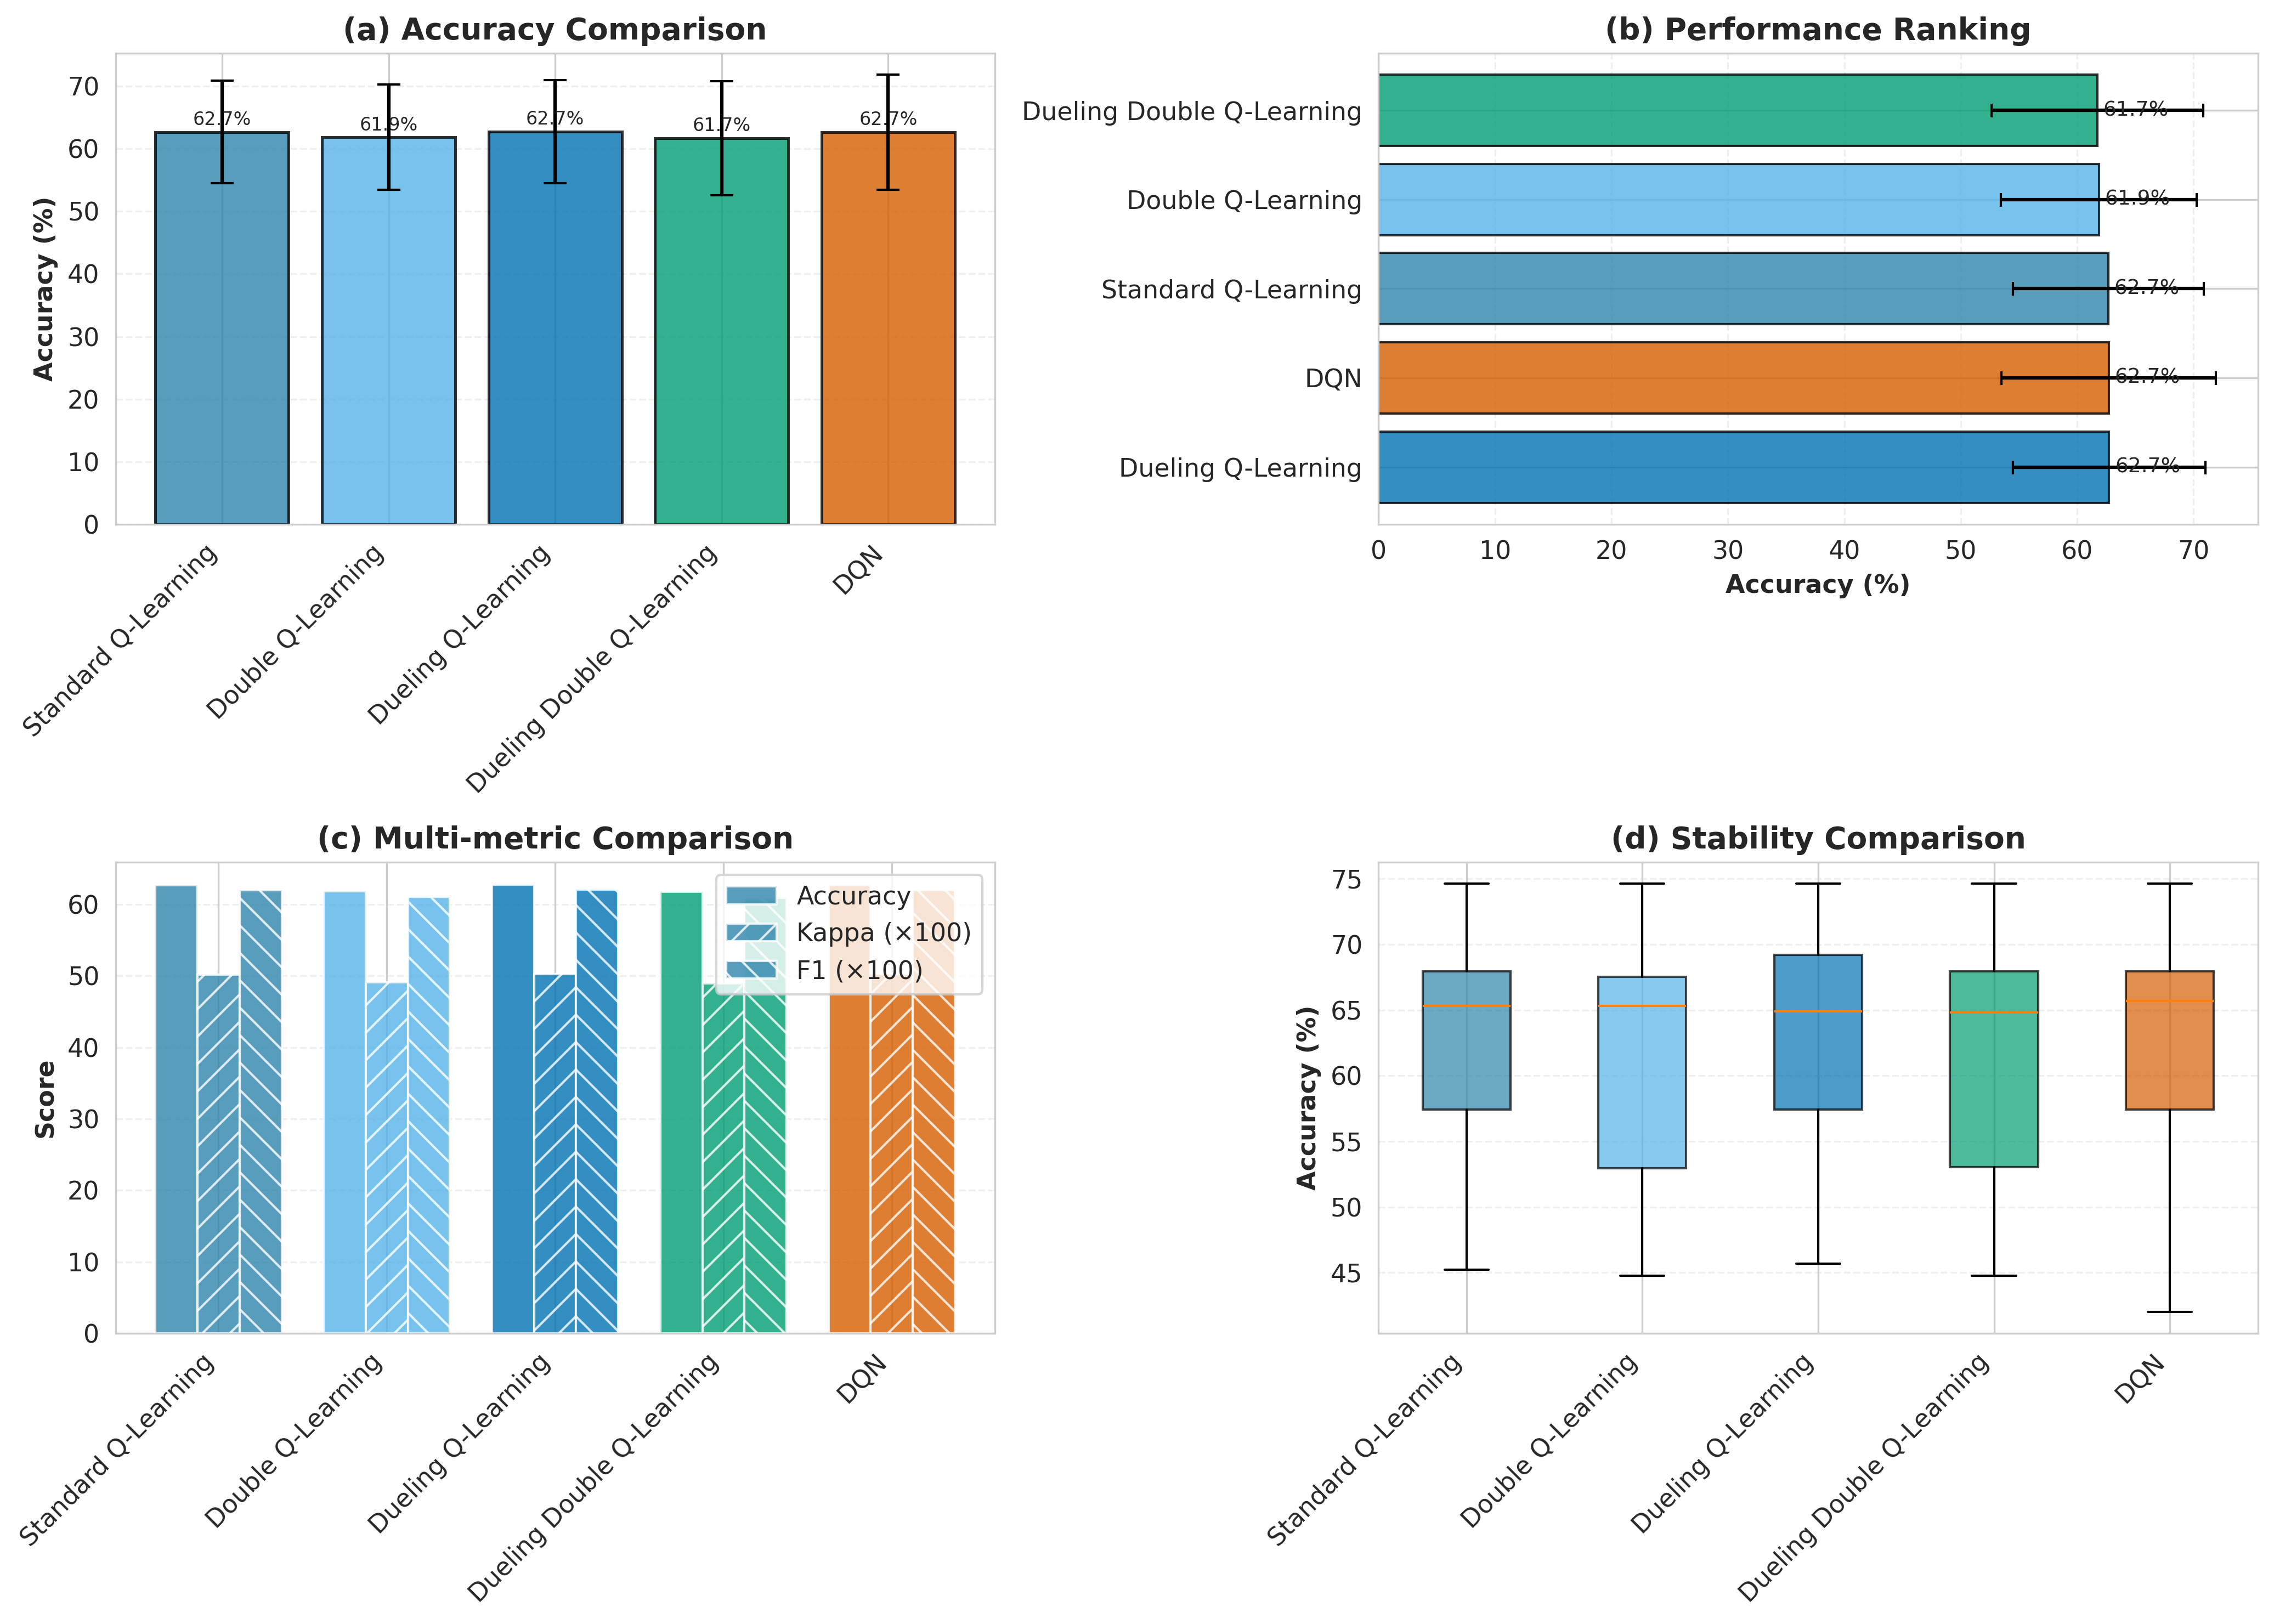
\includegraphics[width=1.0\textwidth]{figures/q_internal/03_performance_comparison.png}
\caption{\textbf{Q-Learning 不同变体的性能对比分析。}}
\label{fig:tableq_dqn_comparison}
\end{figure}

\textbf{(a)} 分类准确率对比。各变体性能高度接近（61.7\%--62.7\%），Standard Q-Learning、Dueling Q-Learning 和 DQN 并列最佳（62.7\%）。

\textbf{(b)} 性能排名。进一步确认了 Standard Q-Learning 等三种方法的领先地位，Dueling Double Q-Learning 略低（61.7\%）。

\textbf{(c)} 多指标综合对比（Accuracy, Kappa, F1）。所有变体在各项指标上表现一致，未见特定变体在某项指标上有显著优势。

\textbf{(d)} 稳定性对比箱线图。各方法的准确率分布范围和中位数基本重合，表明不同 Q-Learning 架构改进对模型稳定性的影响有限。

结果表明，在本任务中，\textbf{Standard Q-Learning 已足以捕捉时间窗口选择的策略，复杂的变体改进（如 Double Q-Learning 或 Dueling 架构）并未带来显著的性能增益}，反而可能增加计算复杂度。

图~\ref{fig:tableq_dqn_detailed} 从多个维度系统评估了五种 Q-Learning 变体的性能。
\begin{figure}[H]
\centering
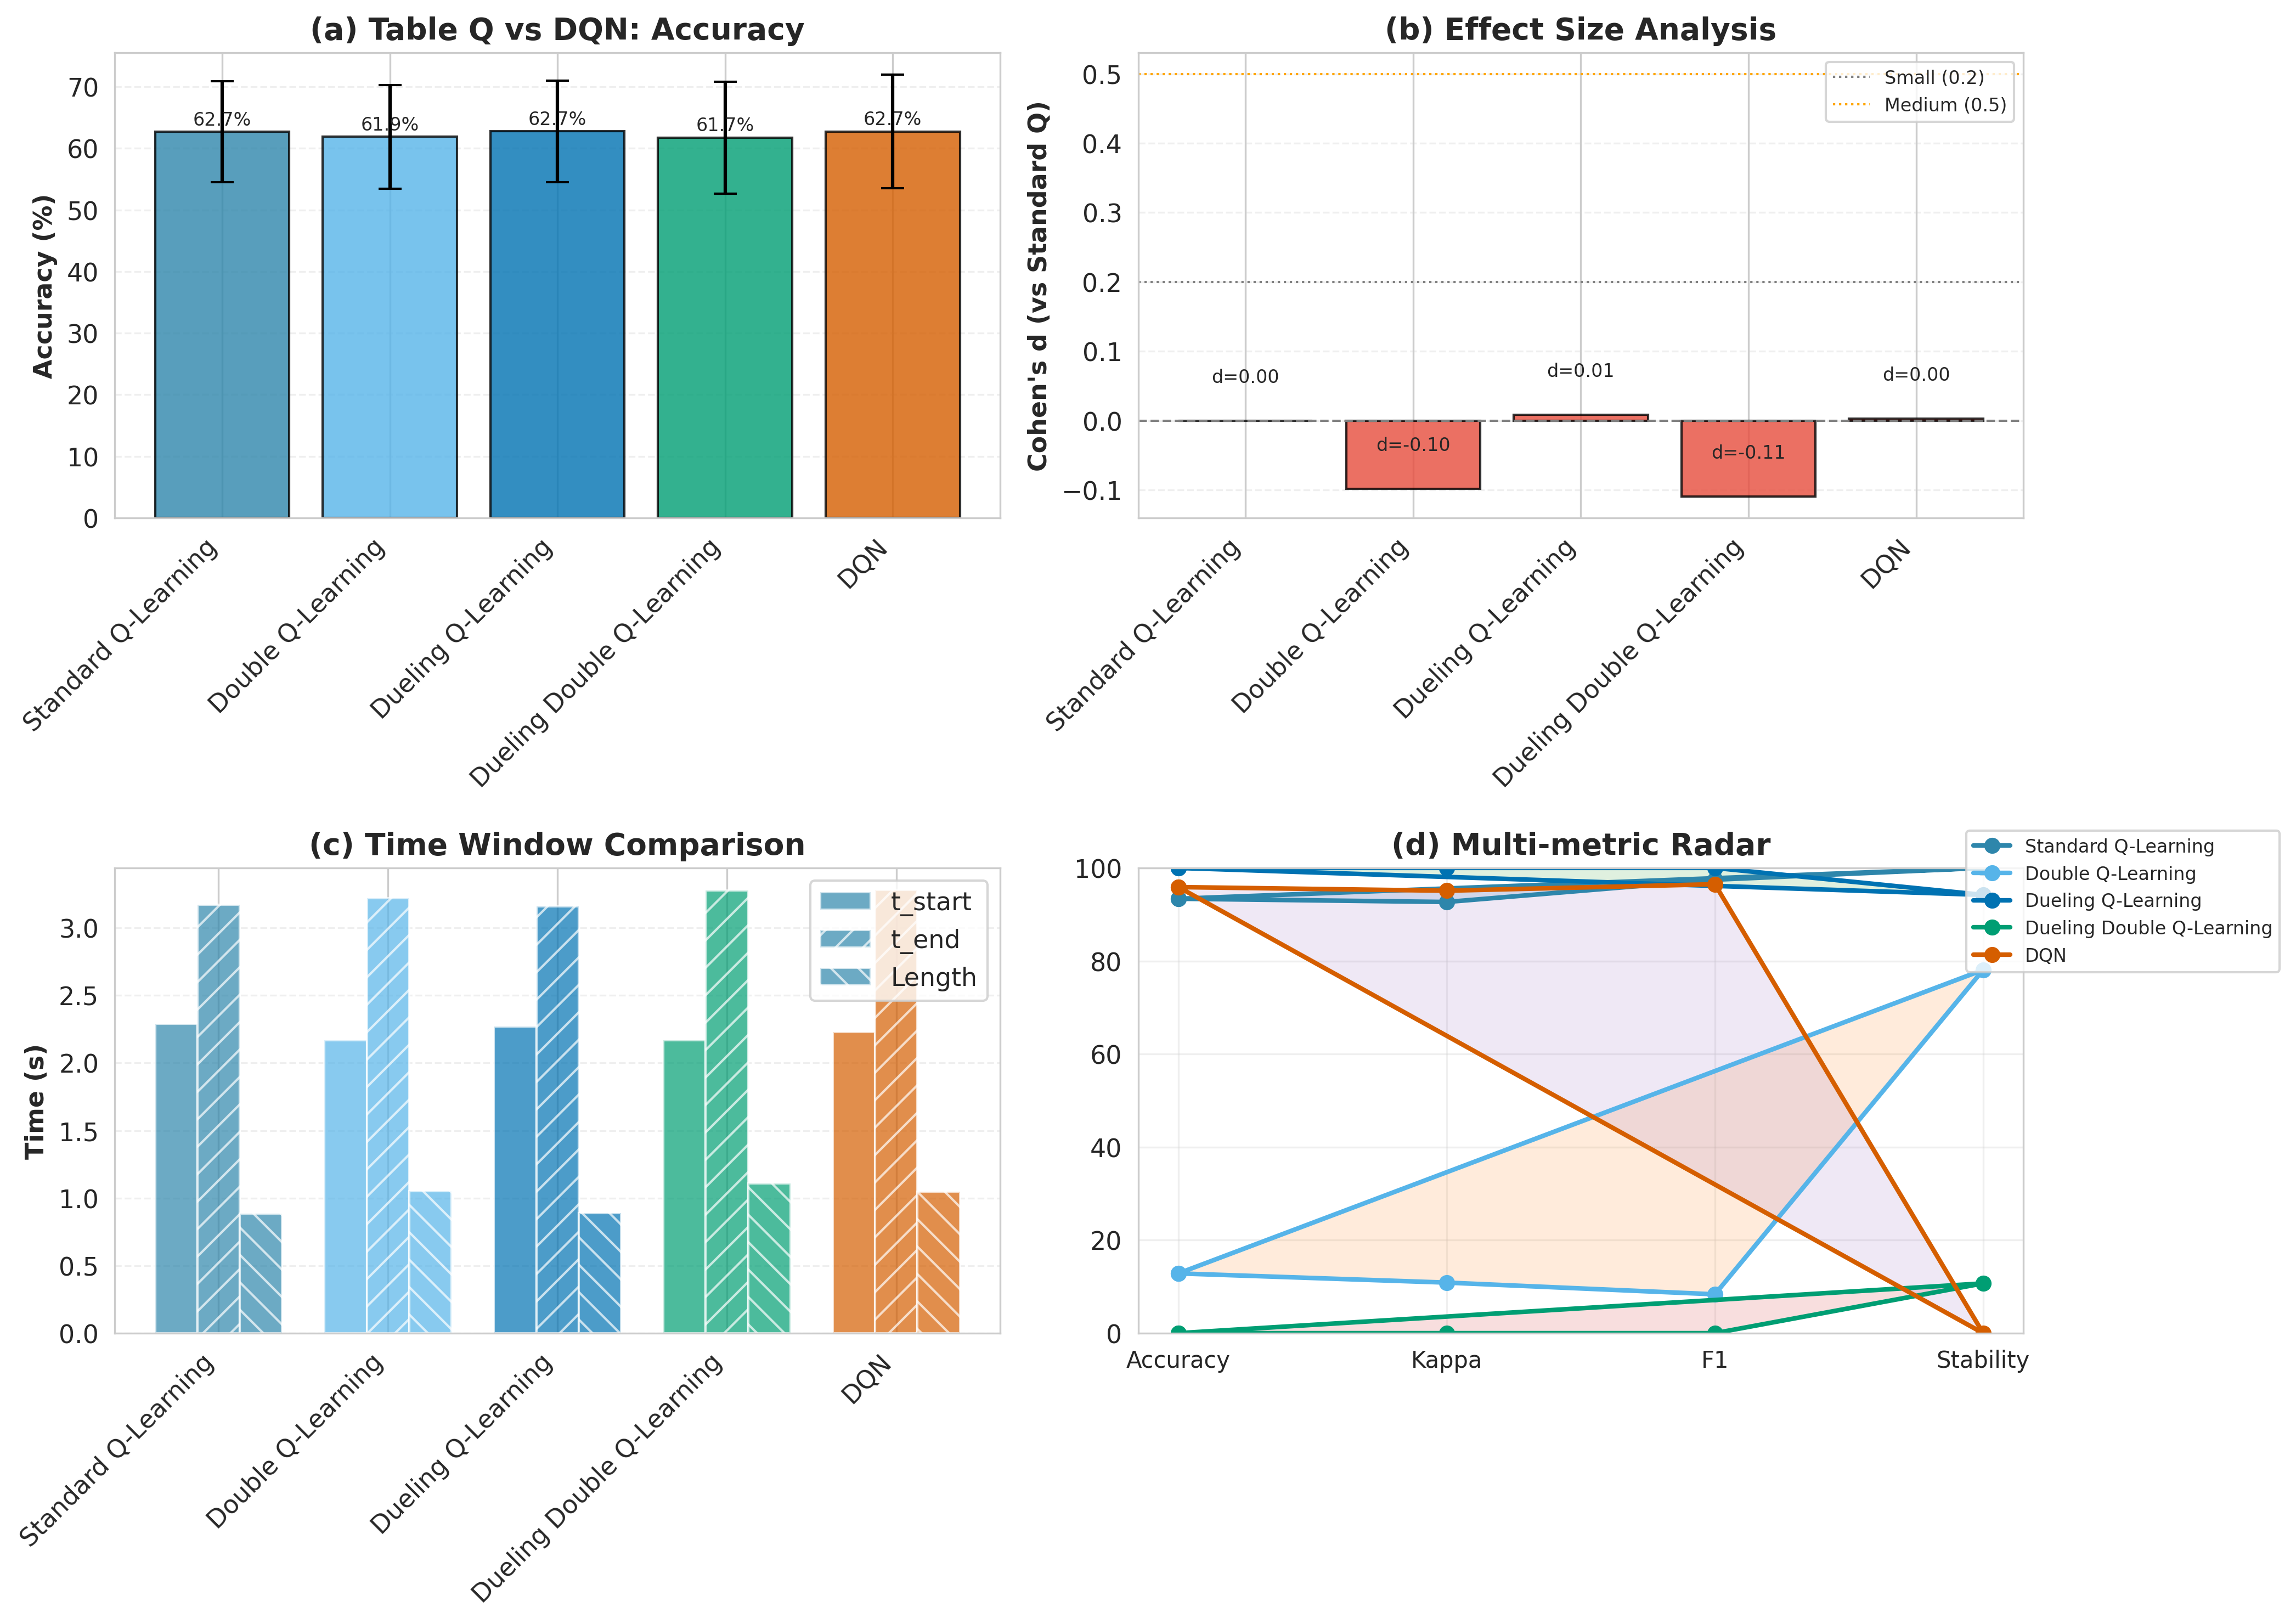
\includegraphics[width=1.0\textwidth]{figures/q_internal/03_table_q_vs_dqn.png}
\caption{\textbf{Table Q-Learning 与 DQN 的深度对比分析。}}
\label{fig:tableq_dqn_detailed}
\end{figure}

本图从准确率、效应量、时间窗口选择和综合指标四个维度系统比较了传统 Table Q-Learning 方法（Standard, Double, Dueling, Dueling Double）与深度学习方法（DQN）的性能。

\textbf{(a)} 分类准确率对比。所有方法性能高度接近（61.7\%--62.7\%），Standard Q-Learning、Dueling Q-Learning 和 DQN 均达到 62.7\% 的最高准确率，Double Q-Learning 略低（61.9\%）。

\textbf{(b)} 效应量分析（Cohen's d），以 Standard Q 为基准。所有方法的效应量均远低于小效应阈值（$|d| < 0.2$），其中 Double Q-Learning ($d=-0.10$) 和 Dueling Double Q-Learning ($d=-0.11$) 显示出微小的负效应，而 Standard Q-Learning ($d=0.00$)、Dueling Q-Learning ($d=0.01$) 和 DQN ($d=0.00$) 与基准几乎无差异。

\textbf{(c)} 时间窗口选择对比，展示各方法的起始时间 ($t_{start}$)、结束时间 ($t_{end}$) 和窗口长度 (Length)。观察发现，DQN 倾向于选择较短的窗口（约 1.0s），起始于 2.2s 左右；而 Table Q-Learning 变体的窗口长度分布在 0.9s--1.1s 之间，起始时间在 2.2s--2.3s。

\textbf{(d)} 多指标雷达图，综合展示准确率、Kappa 系数、F1 分数和稳定性。所有方法在准确率和 F1 指标上表现相近，但在稳定性指标上存在一定差异。

结果表明，\textbf{在本任务中，简单的 Table Q-Learning 与复杂的 DQN 性能相当}，说明状态空间离散化策略已足够有效，深度神经网络的优势未能充分体现，可能由于任务复杂度较低或训练数据有限。

图~\ref{fig:training_performance} 评估了不同 Q-Learning 架构在时间窗口选择任务上的学习效率和稳定性。
\begin{figure}[H]
\centering
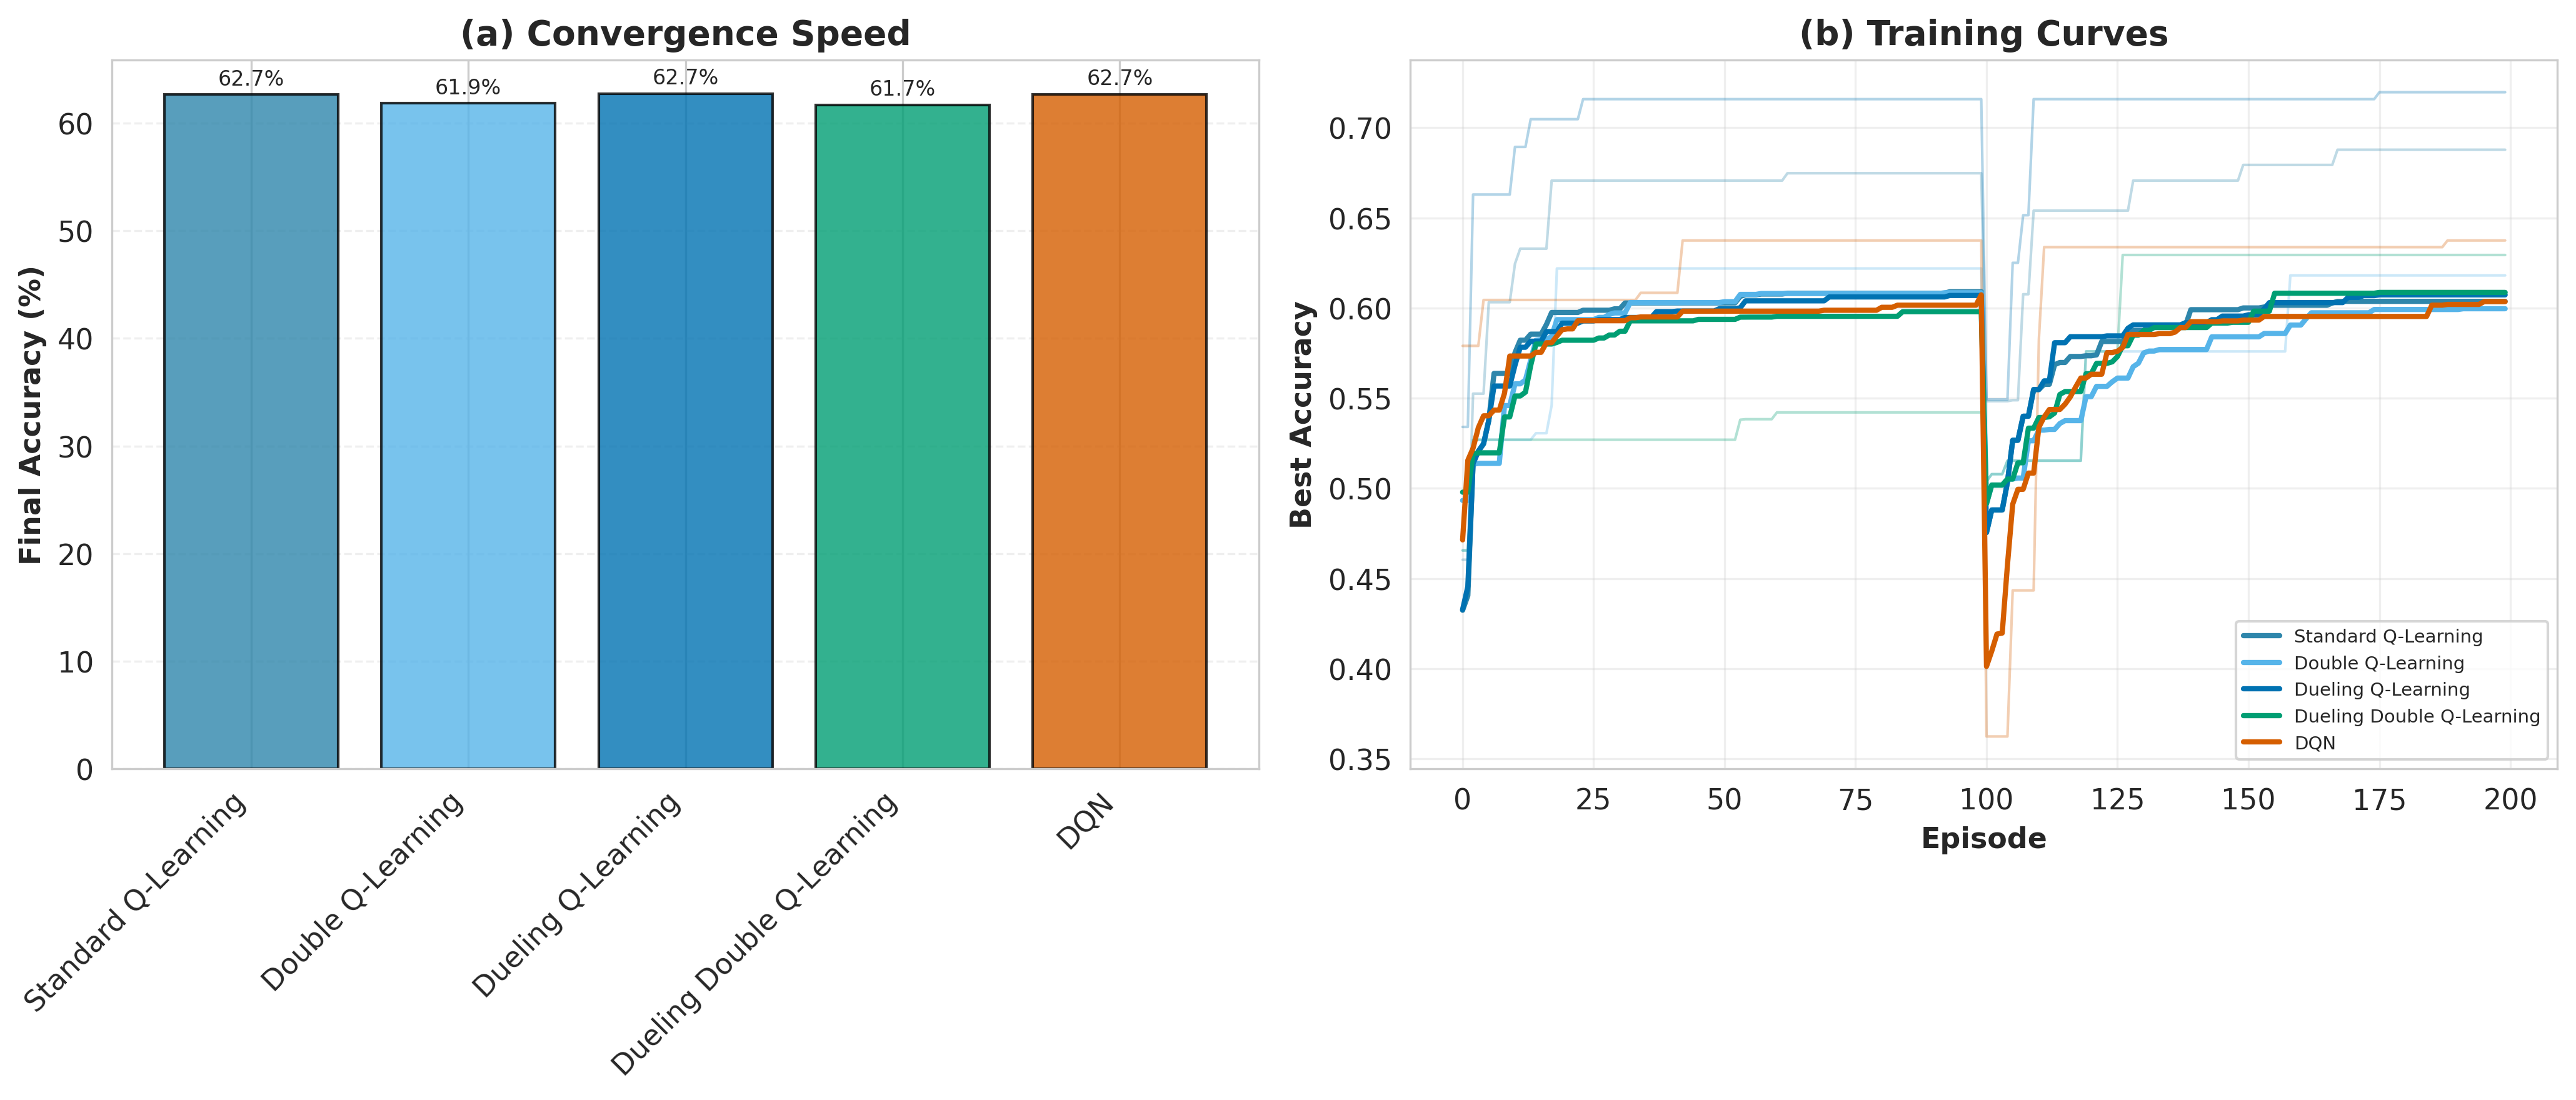
\includegraphics[width=1.0\textwidth]{figures/q_internal/03_training_performance.png}
\caption{\textbf{Q-Learning 变体的收敛特性与训练动态分析。}}
\label{fig:training_performance}
\end{figure}

\textbf{(a)} 最终准确率对比。Standard Q-Learning、Dueling Q-Learning 和 DQN 均达到 62.7\% 的最高性能，Double Q-Learning 及其变体略低（61.7\%--61.9\%），表明复杂架构并未带来最终性能的显著提升。

\textbf{(b)} 训练学习曲线（200 Episodes）。所有方法在初始阶段（0--50 Episodes）均表现出快速收敛特性，准确率迅速攀升至 60\% 左右。在 Episode 100 处观察到的性能波动（可能源于实验协议中的策略重置或环境参数调整）后，各方法均能迅速恢复并趋于稳定。细线表示独立运行轨迹，粗线表示平均趋势。观察发现，Double Q-Learning 显示出较大的训练方差（细线离散度高），而 Standard Q-Learning 和 DQN 表现出更平滑、稳定的收敛过程。

结果表明，Standard Q-Learning 在保持高性能的同时，具有更优的训练稳定性和收敛效率。

表~\ref{tab:tableq_dqn_comparison} 展示了两种方法的详细对比结果。

\begin{table}[H]
\centering
\caption{表格型 Q-Learning 与 DQN 整体性能对比}
\label{tab:tableq_dqn_comparison}
\small
\begin{tabular}{lcccccc}
\hline
\textbf{Method} & \textbf{Accuracy (\%)} & \textbf{Kappa} & \textbf{F1} & \textbf{Std Dev (\%)} & \textbf{Window (s)} \\
\hline
Standard Q-Learning & \textbf{62.68 $\pm$ 8.20} & 0.5019 $\pm$ 0.1114 & 0.6201 $\pm$ 0.0869 & \textbf{8.20} & 0.88 \\
DQN & \textbf{62.70 $\pm$ 9.21} & 0.5022 $\pm$ 0.1251 & 0.6200 $\pm$ 0.0970 & 9.21 & 1.05 \\
\textbf{$\Delta$ (Q - DQN)} & \textbf{-0.02} & -0.0003 & +0.0001 & \textbf{-1.01} & \textbf{-0.17} \\
\hline
\end{tabular}
\end{table}

\textbf{综合以上结果分析如下}：

\textbf{（1）}准确率差异极小：Standard Q-Learning 取得 62.68\% 的准确率，DQN 取得 62.70\% 的准确率，两者差异仅为 -0.02\%，在统计学上可忽略不计。

\textbf{（2）}稳定性优势：Standard Q-Learning 的标准差（8.20\%）低于 DQN（9.21\%），相对降低约 10.97\%。

\textbf{（3）}时间窗选择差异：Standard Q-Learning 选择的时间窗为 $[2.29\text{ s}, 3.17\text{ s}]$（窗口长度 0.88 s），DQN 选择的时间窗为 $[2.23\text{ s}, 3.28\text{ s}]$（窗口长度 1.05 s）。表格型方法倾向于选择更短但信息密度更高的时间窗。

\xmusubsection{被试级别性能对比}{Subject-Level Performance Comparison}
\label{subsec:subject_level_comparison}

表~\ref{tab:subject_comparison} 展示了两种方法在各被试上的详细性能对比。

\begin{table}[H]
\centering
\caption{表格型 Q-Learning 与 DQN 被试级别性能对比}
\label{tab:subject_comparison}
\small
\begin{tabular}{lcccccc}
\hline
\textbf{Subject} & \textbf{Table Q Acc (\%)} & \textbf{DQN Acc (\%)} & \textbf{$\Delta$ Acc (\%)} & \textbf{Table Q Kappa} & \textbf{DQN Kappa} & \textbf{$\Delta$ Kappa} \\
\hline
S01 & 64.47 $\pm$ 2.35 & 65.71 $\pm$ 0.63 & -1.24 & 0.5260 $\pm$ 0.0313 & 0.5435 $\pm$ 0.0084 & -0.0175 \\
S02 & 58.37 $\pm$ 1.85 & 56.74 $\pm$ 2.58 & +1.63 & 0.4780 $\pm$ 0.0247 & 0.4233 $\pm$ 0.0344 & +0.0547 \\
S03 & 68.89 $\pm$ 3.70 & 71.70 $\pm$ 0.37 & -2.81 & 0.5849 $\pm$ 0.0493 & 0.6226 $\pm$ 0.0049 & -0.0377 \\
S04 & 51.91 $\pm$ 1.89 & 51.15 $\pm$ 1.52 & +0.76 & 0.3590 $\pm$ 0.0252 & 0.3469 $\pm$ 0.0203 & +0.0121 \\
S05 & 65.42 $\pm$ 0.63 & 65.27 $\pm$ 0.63 & +0.15 & 0.5389 $\pm$ 0.0084 & 0.5368 $\pm$ 0.0084 & +0.0021 \\
S06 & 47.03 $\pm$ 1.85 & 45.21 $\pm$ 1.83 & +1.82 & 0.2952 $\pm$ 0.0247 & 0.2625 $\pm$ 0.0244 & +0.0327 \\
S07 & 65.46 $\pm$ 0.19 & 65.61 $\pm$ 0.30 & -0.15 & 0.5395 $\pm$ 0.0025 & 0.5416 $\pm$ 0.0040 & -0.0021 \\
S08 & 73.56 $\pm$ 1.31 & 74.62 $\pm$ 0.00 & -1.06 & 0.6470 $\pm$ 0.0175 & 0.6611 $\pm$ 0.0000 & -0.0141 \\
S09 & 68.69 $\pm$ 1.06 & 68.27 $\pm$ 0.85 & +0.42 & 0.5824 $\pm$ 0.0141 & 0.5769 $\pm$ 0.0113 & +0.0055 \\
\hline
\end{tabular}
\end{table}

进一步分析发现：（1）性能优劣分布均衡：在 9 名被试中，表格型 Q-Learning 在 5 名被试（S02、S04、S05、S06、S09）上优于或持平于 DQN，在 4 名被试（S01、S03、S07、S08）上略低于 DQN。（2）低表现被试上的优势：在 S06 被试（低表现组）上，表格型 Q-Learning 取得 47.03\% 的准确率，优于 DQN 的 45.21\%（$\Delta = +1.82\%$）。（3）高表现被试上的差距：在 S03 和 S08 被试（高表现组）上，DQN 略优于表格型方法，但差距在可接受范围内（$< 3\%$）。

\xmusubsection{统计显著性检验}{Statistical Significance Testing}
\label{subsec:statistical_test}

为验证两种方法性能差异的统计显著性，对 9 名被试的准确率进行配对样本 $t$ 检验\cite{field2013discovering}。

\textbf{检验假设}：零假设 $H_0$：$\mu_d = 0$（两种方法的平均准确率无显著差异），备择假设 $H_1$：$\mu_d \neq 0$（两种方法的平均准确率存在显著差异）。

\textbf{检验结果}：$t$ 统计量 $t(8) = -0.024$，双尾 $p$ 值 $p = 0.981$，95\% 置信区间 $[-2.01\%, 1.97\%]$，Cohen's $d = -0.003$。

\textbf{结果解读}。$p = 0.981 > 0.05$，不能拒绝零假设，表明两种方法的性能差异在统计学上不显著。效应量 $d = -0.003$ 远小于 0.2 的阈值，表明即使存在差异，其实际意义也微乎其微。这一结果从统计学角度支持了本研究的核心主张：\textbf{表格型 Q-Learning 可以在不显著牺牲性能的前提下替代 DQN}。

\xmusubsection{自适应时间窗与固定时间窗对比}{Adaptive vs. Fixed Time Window}
\label{subsec:adaptive_vs_fixed}

表~\ref{tab:adaptive_fixed_s01} 对比了自适应时间窗方法（Standard Q-Learning）与固定长度时间窗方法在 S01 被试上的性能。

\begin{table}[H]
\centering
\caption{自适应时间窗与固定时间窗对比（S01 被试）}
\label{tab:adaptive_fixed_s01}
\small
\begin{tabular}{lcccccc}
\hline
\textbf{Method} & \textbf{$t_{\text{start}}$ (s)} & \textbf{$t_{\text{end}}$ (s)} & \textbf{Window (s)} & \textbf{Accuracy (\%)} & \textbf{Kappa} & \textbf{F1} \\
\hline
FL-1s (best) & 2.5 & 3.5 & 1.0 & 61.54 & 0.4869 & 0.6137 \\
FL-1.5s (best) & 2.5 & 4.0 & 1.5 & 59.34 & 0.4578 & 0.5901 \\
FL-2s (best) & 2.0 & 4.0 & 2.0 & 57.88 & 0.4382 & 0.5776 \\
\textbf{Standard Q-Learning} & \textbf{2.80} & \textbf{3.60} & \textbf{0.80} & \textbf{65.93} & \textbf{0.5457} & \textbf{0.6570} \\
\hline
\end{tabular}
\end{table}

Standard Q-Learning 通过学习为 S01 被试选择最优时间窗 $[2.80\text{ s}, 3.60\text{ s}]$，取得 65.93\% 的准确率，优于所有固定长度时间窗方法的最优候选窗口。这一结果验证了本研究方法的有效性：\textbf{自适应时间窗选择能够根据个体神经响应特性动态调整，在连续状态空间中搜索最优解，而非局限于预定义的离散候选集合}。现有研究表明，时间窗的优化选择对运动想象分类性能具有显著影响，基于搜索或学习的方法能够有效捕捉个体化的时间特征\cite{yang2015time, chen2019dynamic, zhang2021mars}。

\xmusubsection{讨论}{Discussion}
\label{subsec:tableq_dqn_discussion}

本节通过详细对比分析，验证了以下结论：（1）性能等价性：表格型 Q-Learning 与 DQN 的准确率差异仅为 -0.02\%，统计检验表明差异不显著（$p = 0.981$）。（2）稳定性优势：表格型 Q-Learning 的跨被试标准差低于 DQN（8.20\% vs 9.21\%），表明其稳定性更优。（3）被试普适性：在 9 名被试中，表格型 Q-Learning 在超过半数的被试上优于或持平于 DQN，尤其在低表现被试上优势更明显。

\xmusection{Q-Learning 变体消融实验}{Q-Learning Variant Ablation Experiments}
\label{sec:ablation}

\xmusubsection{消融实验结果}{Ablation Experiment Results}
\label{subsec:ablation_results}

为验证 Standard Q-Learning 在本任务中的有效性，本节对比多种 Q-Learning 变体的性能。

图~\ref{fig:ablation} 系统评估了在 Standard Q-Learning 基线（Baseline）基础上引入 Double Q 机制、Dueling 架构以及两者结合（Both）对模型性能的影响。

\begin{figure}[H]
\centering
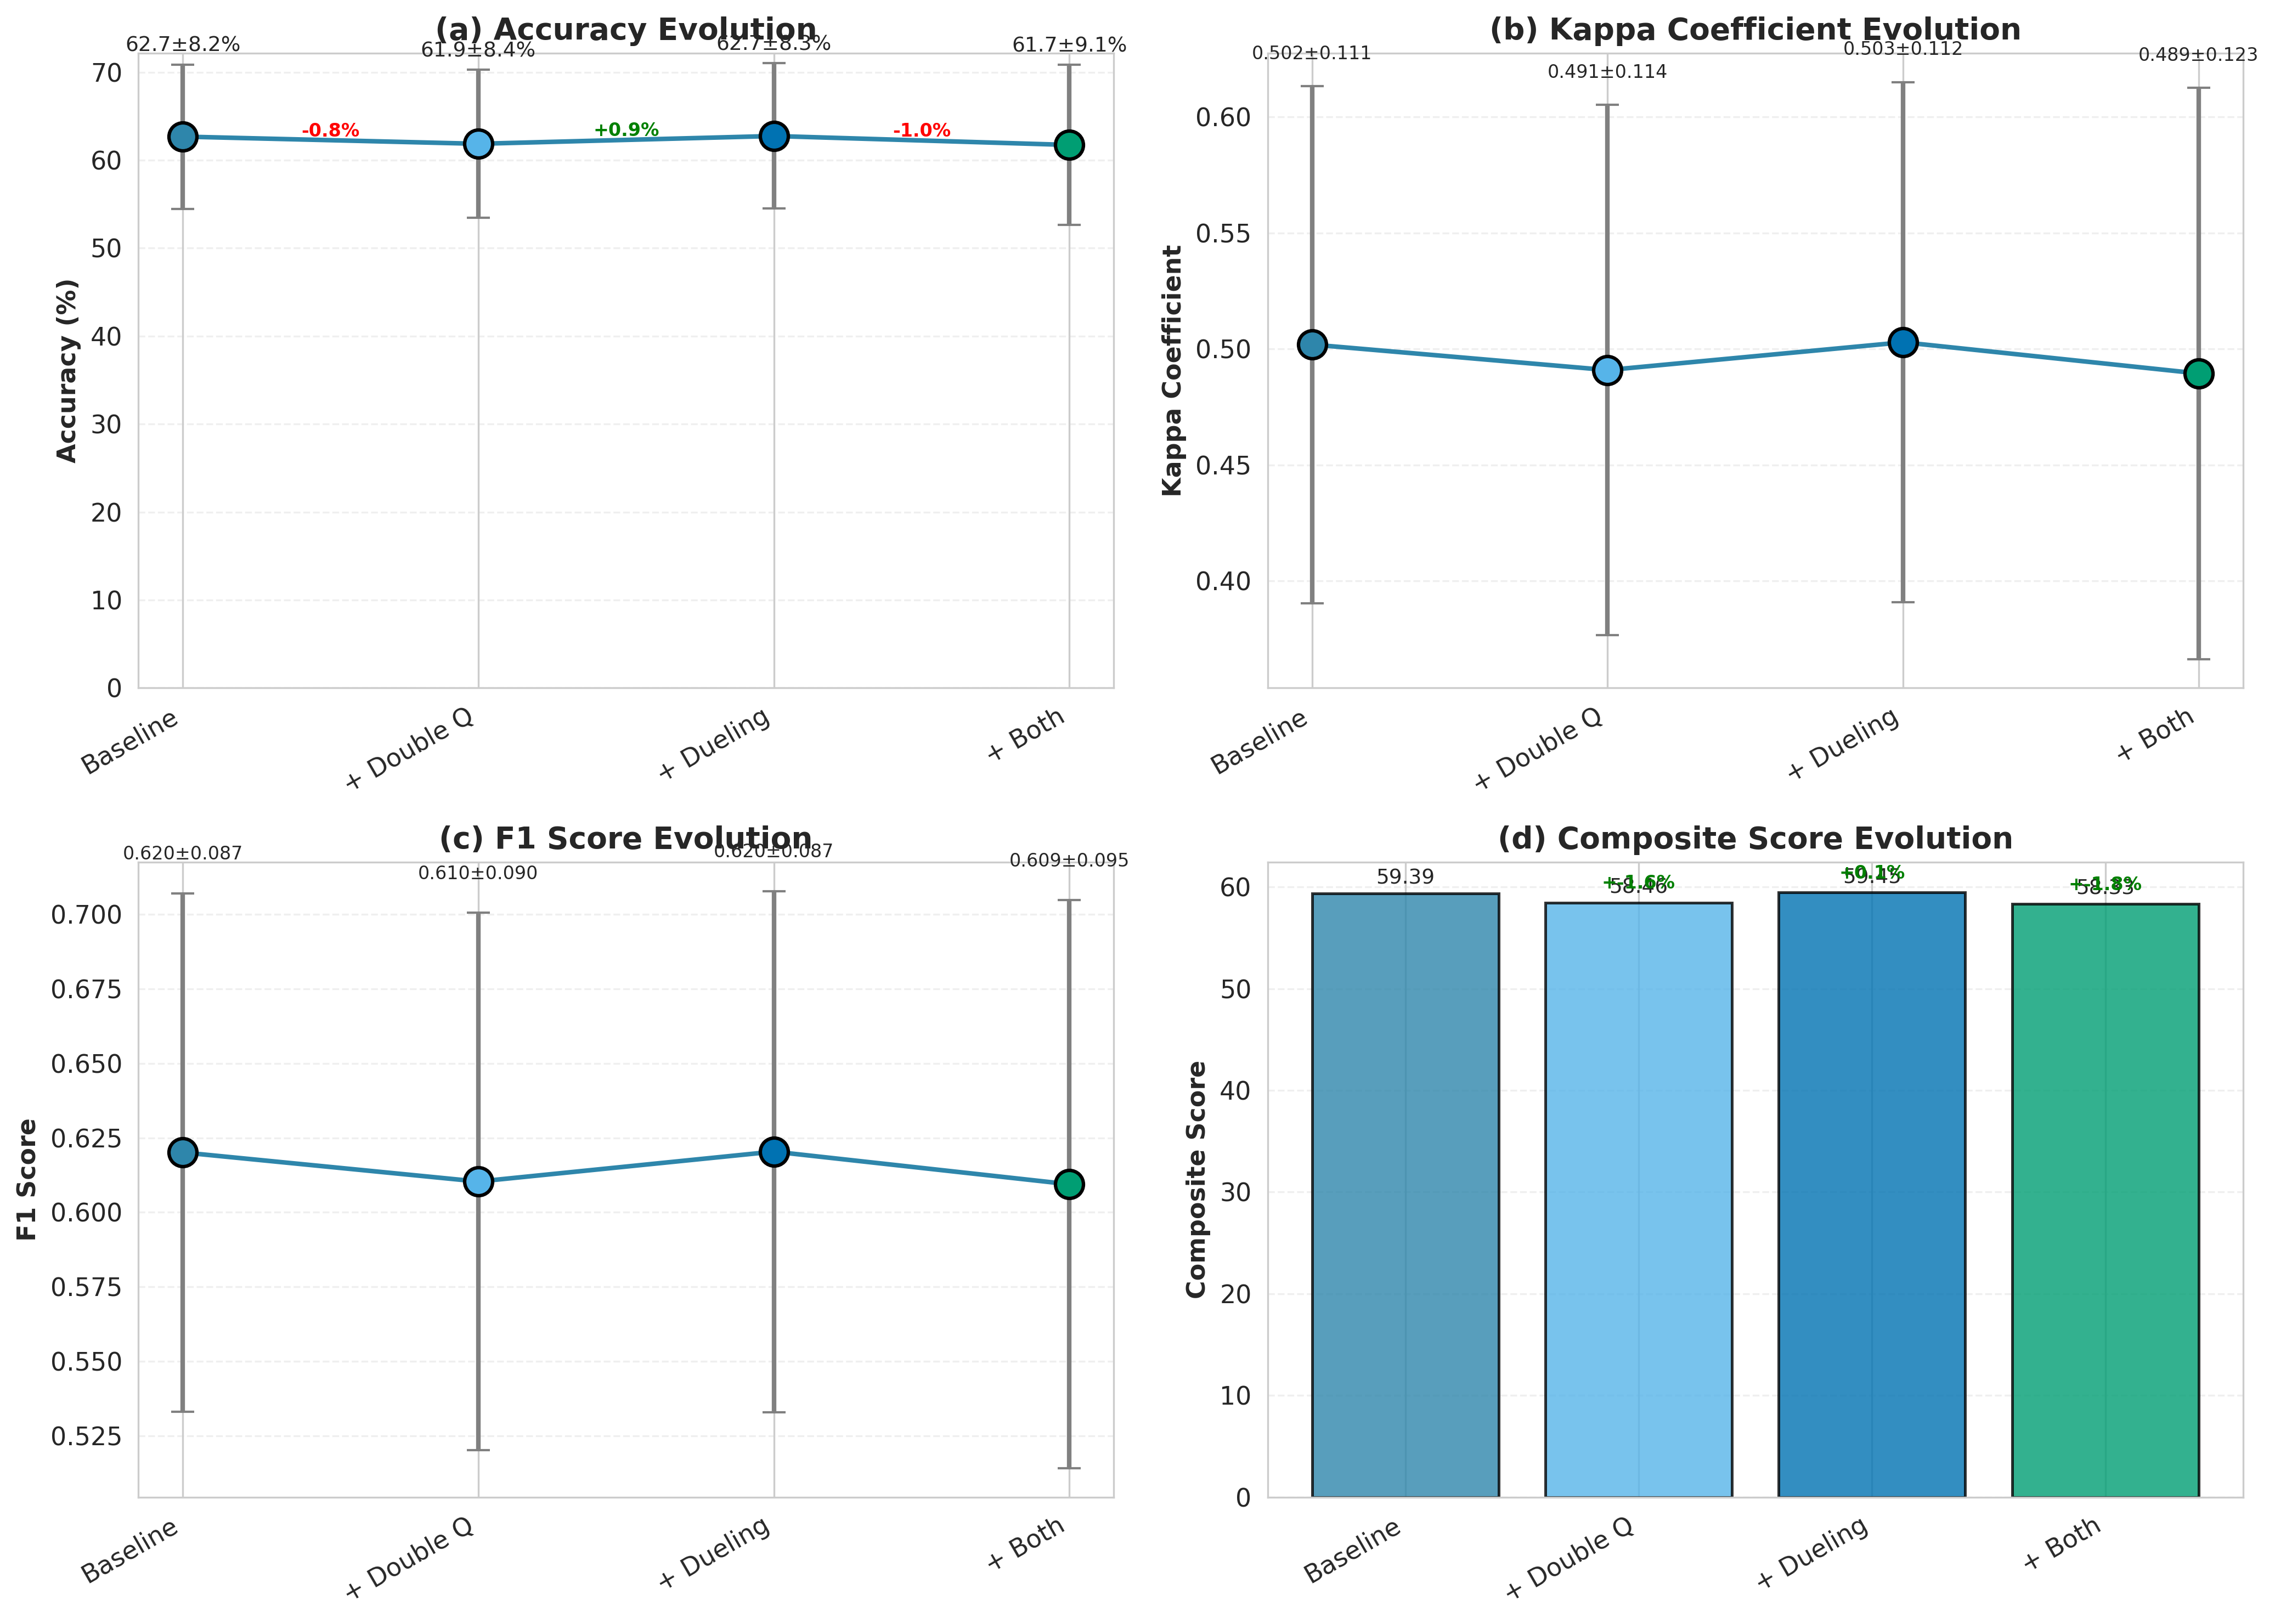
\includegraphics[width=1.0\textwidth]{figures/ablation/04_performance_evolution.png}
\caption{\textbf{Q-Learning 改进策略的消融实验与性能演变分析。}}
\label{fig:ablation}
\end{figure}

\textbf{(a)} 准确率演变。Baseline 准确率为 62.7\%，引入 Double Q 后略微下降至 61.9\% (-0.8\%)，引入 Dueling 架构后恢复至 62.7\% (+0.9\%)，而两者结合（Dueling Double Q-Learning）略降至 61.7\% (-1.0\%)。

\textbf{(b)} Kappa 系数演变。趋势与准确率一致，Baseline (0.502) 与 + Dueling (0.503) 表现最佳，涉及 Double Q 的变体略低（0.491 和 0.489）。

\textbf{(c)} F1 分数演变。Baseline 和 + Dueling 均达到 0.620，而 + Double Q 和 + Both 均为 0.610，表明 Double Q 机制未带来性能增益。

\textbf{(d)} 综合得分对比。Baseline 得分为 59.39，+ Dueling 微增至 59.41，而 + Double Q 和 + Both 分别下降 1.6\% 和 1.8\%。

结果表明，在本任务中，\textbf{Dueling 架构能维持基线性能，但 Double Q 机制并未带来预期收益}，Standard Q-Learning 已是最优选择，复杂的架构改进反而可能引入不必要的计算开销。

图~\ref{fig:window_evolution}深入探究了不同 Q-Learning 变体在时间窗口选择策略上的差异及其对分类性能的影响。
\begin{figure}[H]
\centering
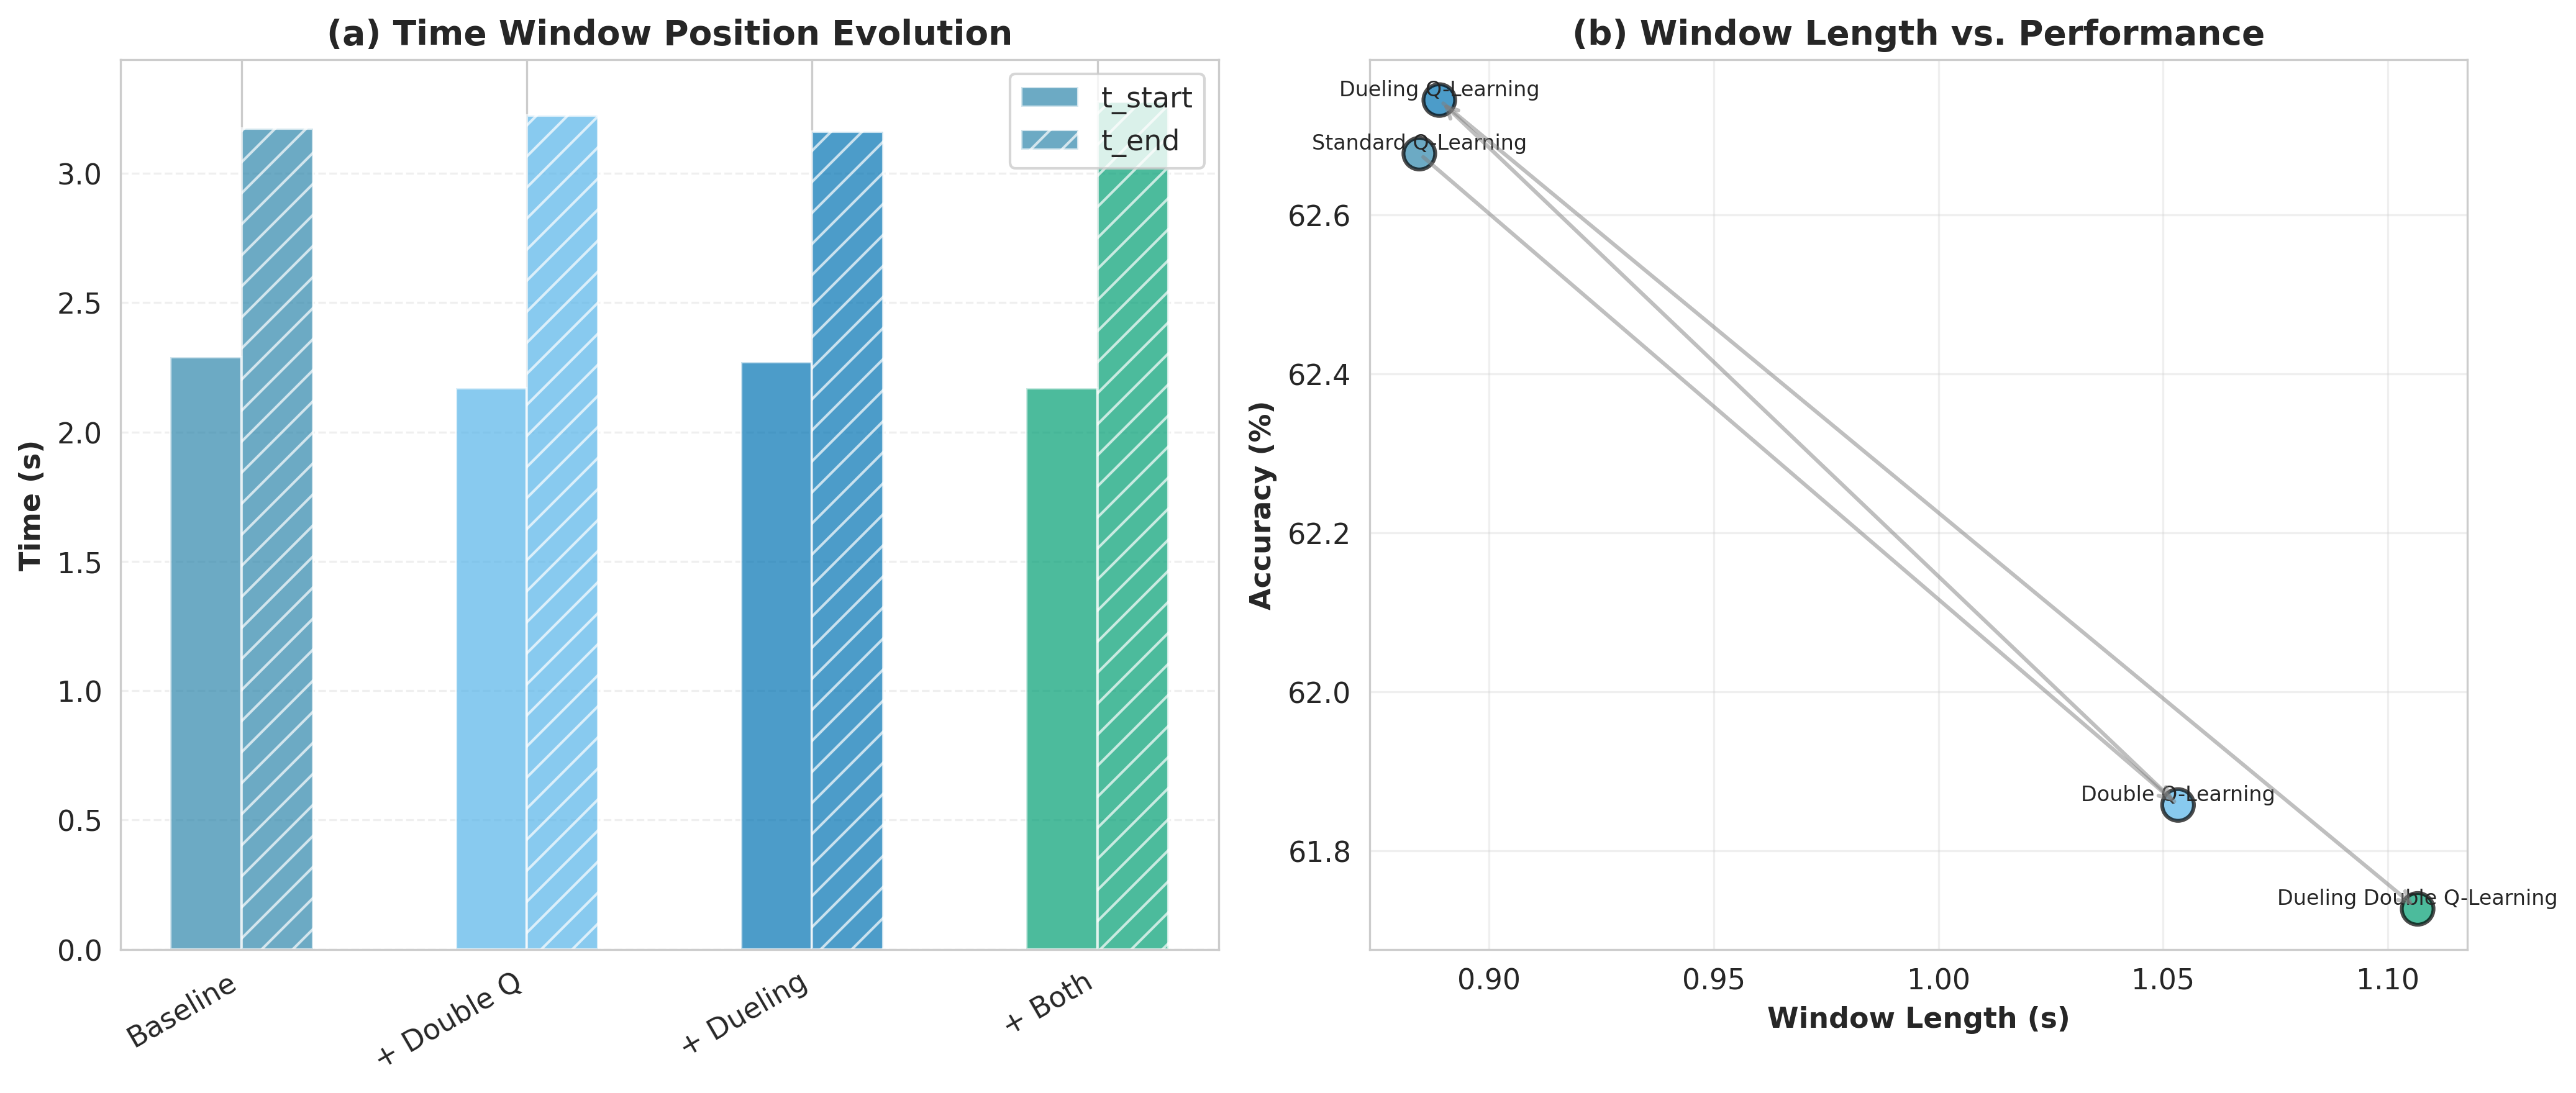
\includegraphics[width=1.0\textwidth]{figures/ablation/04_window_evolution.png}
\caption{\textbf{消融实验中的时间窗口选择模式与性能关系分析。}}
\label{fig:window_evolution}
\end{figure}

\textbf{(a)} 时间窗口位置演变，展示了基线（Baseline）及引入 Double Q、Dueling 架构后的起始时间 ($t_{start}$) 和结束时间 ($t_{end}$)。所有方法均一致地选择试验后期的时间片段（起始约 2.2s，结束约 3.2s--3.3s），验证了运动想象关键特征分布的时间稳定性。

\textbf{(b)} 窗口长度与分类准确率的关系散点图。结果显示显著的负相关趋势：Standard Q-Learning 和 Dueling Q-Learning 选择了较短的窗口（约 0.9s），取得了更高的准确率（62.7\%）；而引入 Double Q 机制的变体（Double Q-Learning, Dueling Double Q-Learning）倾向于选择较长的窗口（1.05s--1.1s），准确率略低（61.7\%--61.9\%）。这表明\textbf{Double Q 机制可能导致代理倾向于更保守的长窗口策略}，从而引入更多噪声，而\textbf{精简的时间窗口（约 0.9s）更有利于捕捉判别性特征并抑制噪声干扰}。

图~\ref{fig:improvement_analysis}从相对提升、效应量、稳定性和分布四个维度深入评估了在 Standard Q-Learning 基线（Baseline）基础上引入 Double Q 机制、Dueling 架构及其组合（Both）的效果。
\begin{figure}[H]
\centering
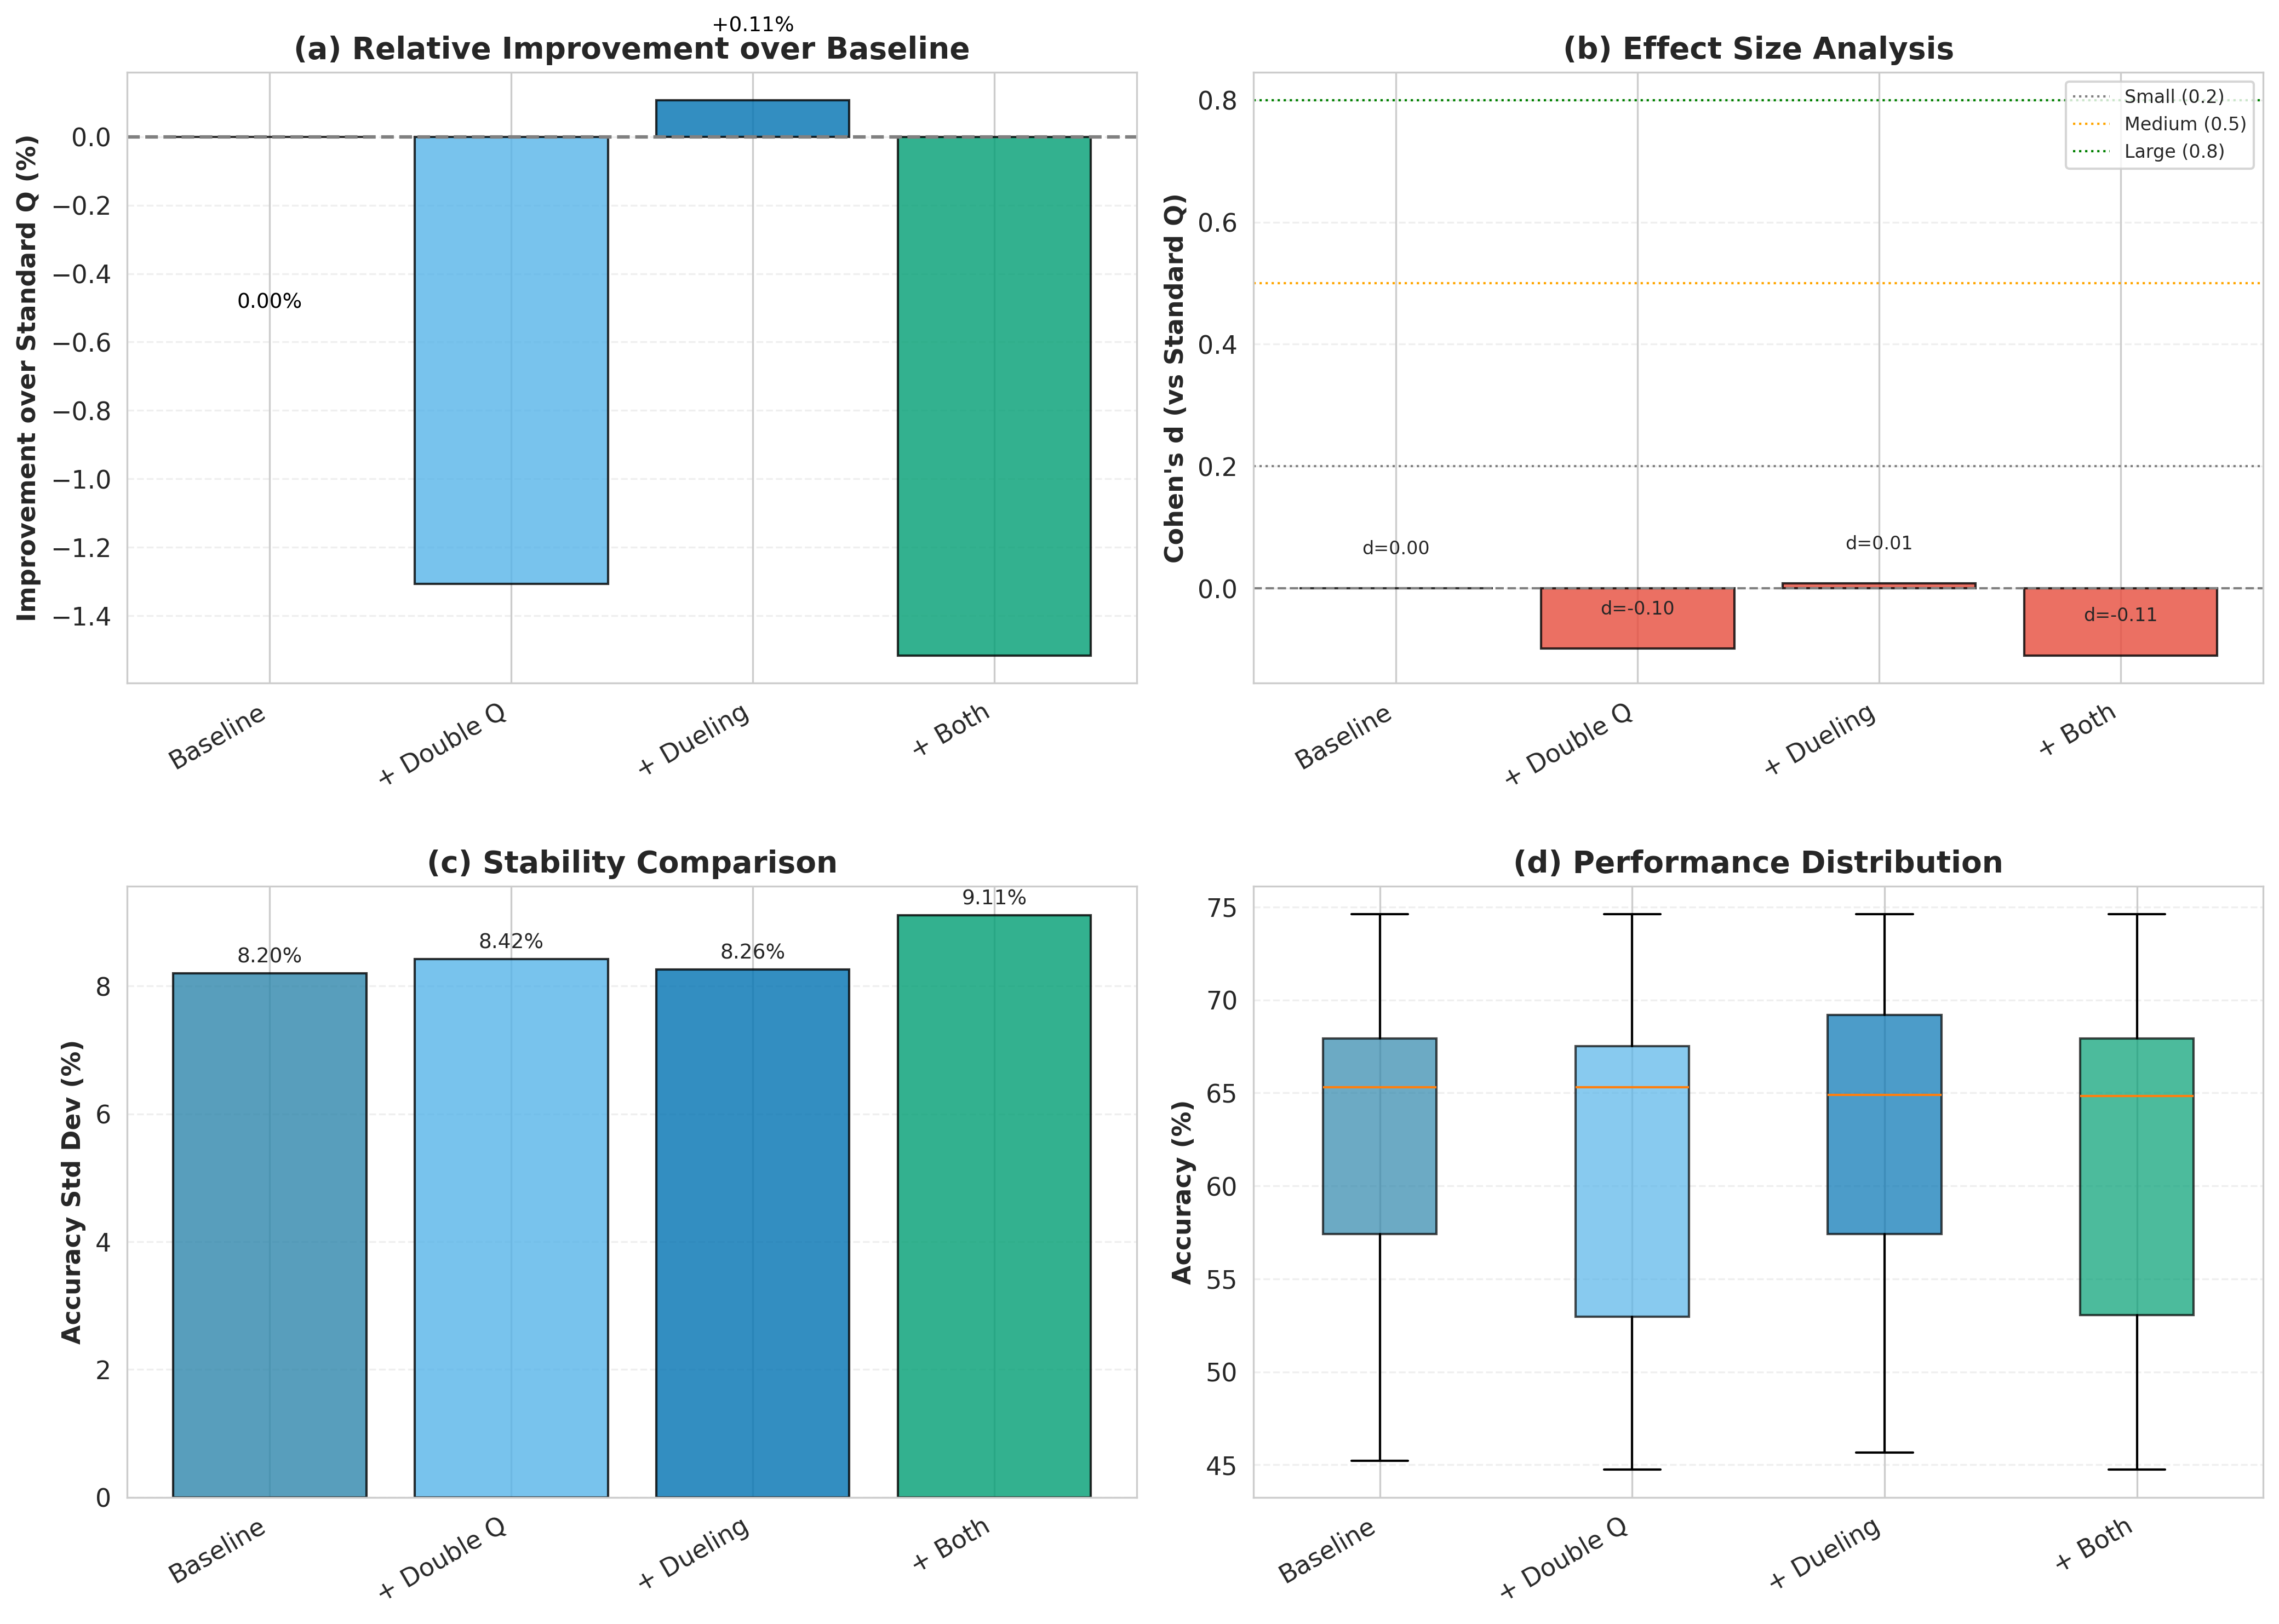
\includegraphics[width=1.0\textwidth]{figures/ablation/04_improvement_analysis.png}
\caption{\textbf{Q-Learning 改进策略的消融实验详细分析。}}
\label{fig:improvement_analysis}
\end{figure}

\textbf{(a)} 相对于基线的性能提升。Dueling 架构带来了微小的正向提升（+0.11\%），而引入 Double Q 机制（-1.3\%）及两者结合（Both, -1.5\%）均导致性能下降。

\textbf{(b)} 效应量分析（Cohen's d）。所有变体与基线的效应量均远小于小效应阈值（$|d| < 0.2$），其中 + Double Q ($d=-0.10$) 和 + Both ($d=-0.11$) 显示出微小的负效应，表明这些改进并未带来统计学上的显著收益。

\textbf{(c)} 稳定性对比（准确率标准差）。Baseline 表现出最佳的稳定性（Std Dev = 8.20\%），而 + Both 的波动性最大（9.11\%），表明复杂的架构组合可能增加了训练的不确定性。

\textbf{(d)} 性能分布箱线图。各方法的中位数相近（约 65\%），但 + Both 的四分位距（IQR）和整体分布范围略宽，进一步印证了其稳定性的下降。

综合分析表明，\textbf{Standard Q-Learning 已足以有效解决本任务的时间窗口选择问题}，引入 Double Q 或 Dueling 等复杂机制不仅未能提升性能，反而可能增加计算复杂度并略微降低稳定性。

表~\ref{tab:ablation} 展示了各 Q-Learning 变体的详细性能对比。

\begin{table}[H]
\centering
\caption{Q-Learning 变体消融实验结果}
\label{tab:ablation}
\small
\begin{tabular}{lcccc}
\hline
\textbf{Method} & \textbf{Accuracy (\%)}  & \textbf{Effect Size ($d$)} & \textbf{Kappa} & \textbf{F1} \\
\hline
\textbf{Standard Q-Learning} & \textbf{62.68 $\pm$ 8.20} & 0.00 & 0.5019 $\pm$ 0.1114 & 0.6201 $\pm$ 0.0869 \\
Double Q-Learning & 61.86 $\pm$ 8.42  & -0.10 & 0.4909 $\pm$ 0.1143 & 0.6103 $\pm$ 0.0901 \\
Dueling Q-Learning & 62.74 $\pm$ 8.26  & 0.01 & 0.5029 $\pm$ 0.1122 & 0.6204 $\pm$ 0.0873 \\
Dueling Double Q-Learning & 61.73 $\pm$ 9.11  & -0.11 & 0.4894 $\pm$ 0.1231 & 0.6094 $\pm$ 0.0952 \\
DQN & 62.70 $\pm$ 9.21  & 0.01 & 0.5022 $\pm$ 0.1251 & 0.6200 $\pm$ 0.0970 \\
\hline
\end{tabular}
\end{table}

\textbf{综合结果分析如下}：

\textbf{（1）}Standard Q-Learning 表现稳健：作为基准方法，Standard Q-Learning 取得了与 DQN 相当的准确率（62.68\% vs 62.70\%），且标准差更低（8.20\% vs 9.21\%）。进一步观察一致性指标，其 Kappa 值（0.5019）与 F1 分数（0.6201）均处于各变体中的最优梯队，表明该策略在分类一致性与正例识别能力上均达到了良好平衡。较低的标准差同时暗示标准算法在本任务的奖励稀疏性与状态转移特性下，具有更优的收敛稳定性，避免了复杂架构可能引入的额外训练噪声。

\textbf{（2）}Double Q-Learning 未带来收益：添加 Double Q-Learning 后准确率下降 1.31\%，效应量 $d = -0.10$。这可能是因为本任务中 Q 值估计的过偏问题不显著，Double Q-Learning 的去偏机制反而导致价值估计过于保守。Double Q-Learning 的核心思想是通过维护两个独立的 Q 函数来缓解过估计问题\cite{van2016deep}，但在本任务的状态空间（136 个离散状态）中，状态 - 动作对的数量有限，Q 值估计的过偏问题并不严重，此时去偏机制可能导致智能体倾向于选择更保守的长窗口策略，从而引入更多噪声。

\textbf{（3）}Dueling 架构效果有限：单独使用 Dueling 架构时准确率微幅提升 0.11\%，但提升不显著。Dueling 架构通过分离状态价值和优势函数来提升性能\cite{wang2016dueling}，但本任务的动作空间较小且状态表征相对简单，各动作间的优势差异本就易于学习，优势函数的显式建模未能带来额外的表征增益。此外，Dueling 架构引入的额外参数可能轻微增加了过拟合风险，抵消了其理论上的表达优势。

\textbf{（4）}组合效果不佳：同时使用 Dueling 与 Double 技术时（Dueling Double Q-Learning），准确率下降 1.52\%，标准差增加至 9.11\%，且 Kappa 与 F1 均为各方法中最低。这表明两种技术的组合未产生协同效应，反而可能因双重机制的耦合导致优化目标冲突：Double Q-Learning 的保守估计倾向与 Dueling 架构的优势敏感机制在梯度更新时产生干扰，增加了训练过程的不稳定性。该结果也印证了“奥卡姆剃刀”原则——在任务复杂度有限的场景下，模型结构的简化往往更利于泛化。

综上，\textbf{Standard Q-Learning 在本任务中是最优选择}，既保持了轻量化优势（参数少、收敛快），又取得了与复杂变体相当甚至更稳定的性能表现。这一结论为后续工程部署提供了重要参考：在状态空间有限、奖励设计合理的中等复杂度任务中，优先采用标准算法并辅以精细的超参数调优，往往比盲目引入高级变体更具性价比。

\xmusubsection{被试间差异分析}{Inter-Subject Difference Analysis}
\label{subsec:subject_variability}

表~\ref{tab:subject_variability} 展示了 Standard Q-Learning 方法在各被试上的性能表现。

\begin{table}[H]
\centering
\caption{Standard Q-Learning 被试间性能差异}
\label{tab:subject_variability}
\footnotesize
\begin{tabular}{lcccccc}
\hline
\textbf{Subject} & \textbf{Accuracy (\%)} & \textbf{Kappa} & \textbf{F1} & \textbf{$t_{\text{start}}$ (s)} & \textbf{$t_{\text{end}}$ (s)} & \textbf{Window (s)} \\
\hline
S01 & 64.47 $\pm$ 2.35 & 0.5260 $\pm$ 0.0313 & 0.6446 $\pm$ 0.0258 & 2.68 & 3.56 & 0.88 \\
S02 & 58.37 $\pm$ 1.85 & 0.4780 $\pm$ 0.0247 & 0.5919 $\pm$ 0.0212 & 2.16 & 2.96 & 0.80 \\
S03 & 68.89 $\pm$ 3.70 & 0.5849 $\pm$ 0.0493 & 0.6889 $\pm$ 0.0405 & 2.36 & 3.72 & 1.36 \\
S04 & 51.91 $\pm$ 1.89 & 0.3590 $\pm$ 0.0252 & 0.5209 $\pm$ 0.0206 & 2.04 & 2.64 & 0.60 \\
S05 & 65.42 $\pm$ 0.63 & 0.5389 $\pm$ 0.0084 & 0.6484 $\pm$ 0.0069 & 2.00 & 2.68 & 0.68 \\
S06 & 47.03 $\pm$ 1.85 & 0.2952 $\pm$ 0.0247 & 0.4415 $\pm$ 0.0202 & 2.00 & 2.88 & 0.88 \\
S07 & 65.46 $\pm$ 0.19 & 0.5395 $\pm$ 0.0025 & 0.6528 $\pm$ 0.0026 & 2.04 & 2.92 & 0.88 \\
S08 & 73.56 $\pm$ 1.31 & 0.6470 $\pm$ 0.0175 & 0.7293 $\pm$ 0.0143 & 2.44 & 3.92 & 1.48 \\
S09 & 68.69 $\pm$ 1.06 & 0.5824 $\pm$ 0.0141 & 0.6784 $\pm$ 0.0115 & 2.68 & 3.36 & 0.68 \\
\hline
\textbf{Mean} & \textbf{62.68} & \textbf{0.5019} & \textbf{0.6201} & \textbf{2.29} & \textbf{3.17} & \textbf{0.88} \\
\textbf{Std} & \textbf{8.20} & \textbf{0.1114} & \textbf{0.0869} & \textbf{0.26} & \textbf{0.46} & \textbf{0.32} \\
\hline
\end{tabular}
\end{table}

\textbf{被试分组分析}。（1）高表现组（S03、S07、S08、S09）：准确率 $> 65\%$，Kappa $> 0.54$。（2）中表现组（S01、S02、S05）：准确率 58\%--65\%，Kappa 0.48--0.54。（3）低表现组（S04、S06）：准确率 $< 52\%$，Kappa $< 0.36$。值得注意的是，所有被试选择的时间窗起始点集中在 2.0 s--2.7 s 范围内，与运动想象任务中 ERD 现象的典型时间特征（刺激后 2 s--4 s）相符\cite{pfurtscheller1999event}，验证了本研究方法的学习有效性。

\xmusection{本章小结}{Chapter Summary}

本章在 BCI Competition IV 2a 标准数据集上系统评估了表格型 Q-Learning 时间窗优化方法的性能，通过多层次、多维度的对比实验得出以下主要结论：

（1）\textbf{自适应策略优于固定策略}：搜索优化方法（Grid-Search 63.35\%、Random-Search 61.95\%）显著优于固定时间窗方法（约 45\%），变异系数降低约 30\%（13.5\%--13.9\% vs 19.8\%--23.9\%），验证了自适应时间窗选择能够有效捕捉个体化的神经响应特征。

（2）\textbf{Q-Learning 与基线方法性能等效}：Standard Q-Learning（62.68\%）和 Dueling Q-Learning（62.74\%）与 Grid-Search（63.35\%）的差距仅为 0.6\%--1.6\%，Cohen's $d$ 效应量远小于小效应阈值（$|d| < 0.2$），统计检验表明差异不显著。更重要的是，Q-Learning 方法在推理阶段仅需单次查表操作，计算效率远优于需要遍历所有候选窗口的 Grid-Search。

（3）\textbf{表格型 Q-Learning 可替代 DQN}：本研究的核心主张得到充分验证——表格型 Q-Learning（62.68\%）与 DQN（62.70\%）的准确率差异仅为 -0.02\%，配对样本 $t$ 检验表明差异在统计学上不显著（$t(8) = -0.024$, $p = 0.981$）。此外，表格型方法的跨被试标准差更低（8.20\% vs 9.21\%），且在 9 名被试中的 5 名上优于或持平于 DQN，尤其在低表现被试（S06）上优势更明显（+1.82\%）。

（4）\textbf{Standard Q-Learning 为最优选择}：消融实验表明，Double Q-Learning（-1.31\%）和 Dueling Double Q-Learning（-1.52\%）均未带来性能增益，反而因过于保守的价值估计导致性能下降。Dueling 架构虽维持基线性能（+0.11\%），但提升不显著。Standard Q-Learning 以其简洁性和稳健性成为本任务的最优选择。

（5）\textbf{时间窗选择模式具有神经生理学一致性}：所有方法均倾向于选择试验后期的时间片段（$t_{\text{start}} \approx 2.2$ s，$t_{\text{end}} \approx 3.3$ s），且窗口长度与性能呈负相关趋势（较短窗口约 0.9 s 比较长窗口>1.0 s 准确率更高），与 ERD 现象的典型时间特征相符，验证了本研究方法的学习有效性。

本章实验的局限性在于：（1）仅在 9 名健康被试的标准数据集上验证，未在真实患者群体或在线 BCI 系统中测试；（2）计算效率分析仅基于理论复杂度，未进行实际运行时间的基准测试；（3）未探索迁移学习策略，跨 session 或跨被试的泛化能力有待进一步研究。这些局限性为未来研究指明了方向，将在第 5 章总结与展望中进行详细讨论。